\documentclass[10pt]{article} % For LaTeX2e
\usepackage{tmlr}
% If accepted, instead use the following line for the camera-ready submission:
%\usepackage[accepted]{tmlr}
% To de-anonymize and remove mentions to TMLR (for example for posting to preprint servers), instead use the following:
%\usepackage[preprint]{tmlr}

% Optional math commands from https://github.com/goodfeli/dlbook_notation.
\input{math_commands.tex}

\usepackage{hyperref}
\usepackage{url}

\usepackage{graphicx}
\usepackage{tikz}
\usepackage{xcolor}
\usepackage{listings}
\usepackage{algorithm}
\usepackage{algorithmic}
\usepackage{soul}
\usepackage{multicol}
\usepackage{multirow}
\usepackage{adjustbox}
\usepackage{booktabs}
\usepackage{tcolorbox}
\usepackage{array}
\usepackage{colortbl}
\usepackage{longtable}
\usepackage[table,xcdraw]{xcolor}
\usepackage{ltablex}
\usepackage[normalem]{ulem}
\usepackage{longtable}
\usepackage{amsmath}


\title{Enhancing Large Language Models for Constraint-Driven Molecular
Generation and Beyond}

% Authors must not appear in the submitted version. They should be hidden
% as long as the tmlr package is used without the [accepted] or [preprint] options.
% Non-anonymous submissions will be rejected without review.

\author{\name Kyunghyun Cho \email kyunghyun.cho@nyu.edu \\
      \addr Department of Computer Science\\
      University of New York
      \AND
      \name Raia Hadsell \email raia@google.com \\
      \addr DeepMind
      \AND
      \name Hugo Larochelle \email hugolarochelle@google.com\\
      \addr Mila, Universit\'e de Montr\'eal \\
      Google Research\\
      CIFAR Fellow}

% The \author macro works with any number of authors. Use \AND 
% to separate the names and addresses of multiple authors.

\newcommand{\fix}{\marginpar{FIX}}
\newcommand{\new}{\marginpar{NEW}}

\def\month{MM}  % Insert correct month for camera-ready version
\def\year{YYYY} % Insert correct year for camera-ready version
\def\openreview{\url{https://openreview.net/forum?id=XXXX}} % Insert correct link to OpenReview for camera-ready version


\begin{document}


\maketitle

\begin{abstract}
Most de novo molecule generators attempt to satisfy hard chemical constraints in a single forward pass, offering little guidance when outputs fall short. We introduce Code-Driven Molecular Synthesis (CDMS) -- an iterative, model-agnostic framework that embeds a formal self-improving feedback loop into large language models (LLMs). At the start of each task, the LLM uses the chemist’s request as input to generate a snippet of executable code, referred to as an \emph{inspector}, which formalizes the evaluation logic for guiding molecular refinement. This inspector remains fixed throughout the refinement process and is executed on every candidate molecule at each iteration. It produces natural-language critiques describing how to improve the molecule to better meet user-defined constraints (e.g., “add a para-hydroxyl group”). These \emph{Programmatic Feedback Gradients} are appended to subsequent prompts, guiding the LLM toward progressively refined outputs until all structural and functional requirements are satisfied. CDMS achieves state-of-the-art success rates in constraint satisfaction using only a few feedback iterations and without any model retraining. To encourage further research, we release a benchmark dataset curated for code-generated, feedback-driven molecular design
\footnote{\url{https://anonymous.4open.science/r/CDMS-C08D/}}.
\end{abstract}

\section{Introduction}


    \begin{figure}[h]
        \centering
        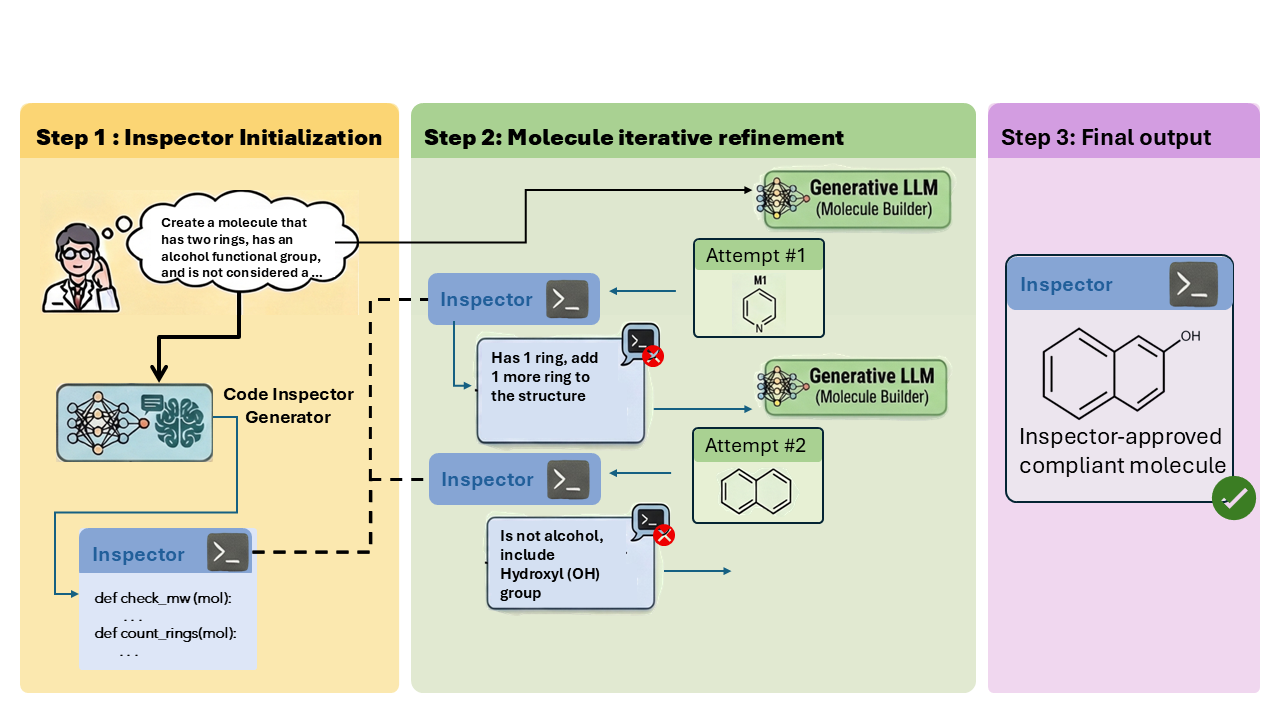
\includegraphics[width=0.6\linewidth]{figures/overview.png}
        \caption{CDMS molecule generation process}
        \label{fig:feedback_example}
    \end{figure}

    De novo molecular design is a complex and multi-stage process. It begins by identifying the desired attributes of a chemical compound, including its molecular structure, properties, and potential applications. Candidate molecules are then evaluated for properties such as chemical validity, predicted synthetic accessibility, drug-likeness, and toxicity~\cite{brown2019guacamol,parrot2023syntheticaccessibility}. Recent advances in deep generative modeling have introduced methods for the de novo generation and optimization of molecular candidates, including goal-directed, property-conditioned, and target-aware approaches~\citep{jin2018junction,you2018graph,hoogeboom2022equivariant,wu2024tamgen}. However, these models may generate molecules that do not adhere to the specified requirements or are impractical to synthesize because of unavailable precursors or overly complex synthesis routes~\cite{gao2020synthesizability}. Therefore, a common computational workflow separates the process into two stages: generating molecules with the potential to meet the specified constraints, followed by ranking or filtering the candidates using classifiers, molecular-property predictors, and synthetic-accessibility estimators~\cite{parrot2023syntheticaccessibility,guo2025synthesizability}. This paper focuses on the first stage: generating molecular candidates that adhere to the desired computable constraints, rather than performing synthesis planning or experimental validation. We demonstrate that CDMS generates candidates with favorable computed synthetic-accessibility and drug-likeness scores~\cite{ertl2009sascore,bickerton2012qed}, and introduce an expert-curated dataset specifically designed for evaluating this task.

    Recently, models that leverage LLMs have demonstrated strong performance on tasks in the natural sciences and cheminformatics, including applications in \textit{de novo} molecule generation~\cite{molregpt,zhang2024chemllm,CIQA}. While LLMs demonstrate substantial knowledge of chemical concepts relevant to molecular design, their ability to reliably satisfy multiple complex, user-defined constraints remains limited. Generating molecules that jointly satisfy functional-group, structural, and physicochemical requirements---which are important in applications such as drug discovery---poses a significant challenge for current generative models~\cite{fu2021mimosa}. For instance, generating a molecule with multiple constraints, such as two aromatic rings, a molecular weight between $150$ and $300$ Da, and a carboxylic acid group, requires joint control over ring systems, functional-group presence, and molecular properties---an area in which current models often fall short.
    
   We address these challenges with a novel framework composed of two components: a generative model that designs molecules and an inspector that validates compliance with user-defined textual constraints via executable code. The inspector plays a central role in an iterative feedback loop by generating \emph{Programmatic Feedback Gradients} -- natural-language signals derived from code execution that guide the model toward satisfying the specified requirements. When constraint violations are detected, such as incorrect stereochemistry or invalid ring structures, the inspector returns actionable textual feedback, which is incorporated into subsequent prompts, progressively refining the generated molecules toward full compliance. Figure~\ref{fig:feedback_example} illustrates the end-to-end feedback loop, and an example of the molecular revision process is shown in Figure~\ref{fig:mol_generation_feedback_example}. This mechanism ensures robust alignment between generated outputs and the target properties.
    
    We collaborated with chemistry and computer science experts to construct a new dataset of molecular-generation constraints, along with corresponding golden inspector code capable of verifying whether generated molecules satisfy the specified requirements. Empirically, we demonstrate that CDMS outperforms all evaluated baselines for constraint-driven molecule generation, including specialized molecular generation models, general-purpose LLMs, and recent iterative refinement methods. Moreover, we provide initial evidence that CDMS is applicable beyond molecular design by evaluating it on two additional natural language processing (NLP) tasks that require strict, constraint-driven generation.
    
The contributions of this work are threefold:
    \textbf{(1)} We introduce a novel framework that combines generative models with a novel Inspector Model capable of producing executable code to iteratively validate outputs against complex requirements. We also show that CDMS can generate molecules that achieve higher constraint-satisfaction rates than previous SOTA models. This iterative feedback loop ensures high precision and robust alignment between generated outputs and user-defined constraints. \textbf{(2)} Leveraging an expert-curated dataset, we empirically demonstrate that CDMS outperforms traditional LLMs and SOTA refinement techniques in molecular generation tasks. \textbf{(3)} We establish the versatility of CDMS by showcasing its successful application to broader NLP tasks requiring constraint-driven generation, highlighting its potential to generalize beyond molecular design into other domains.
    
    \begin{figure*}[h]
        \centering
        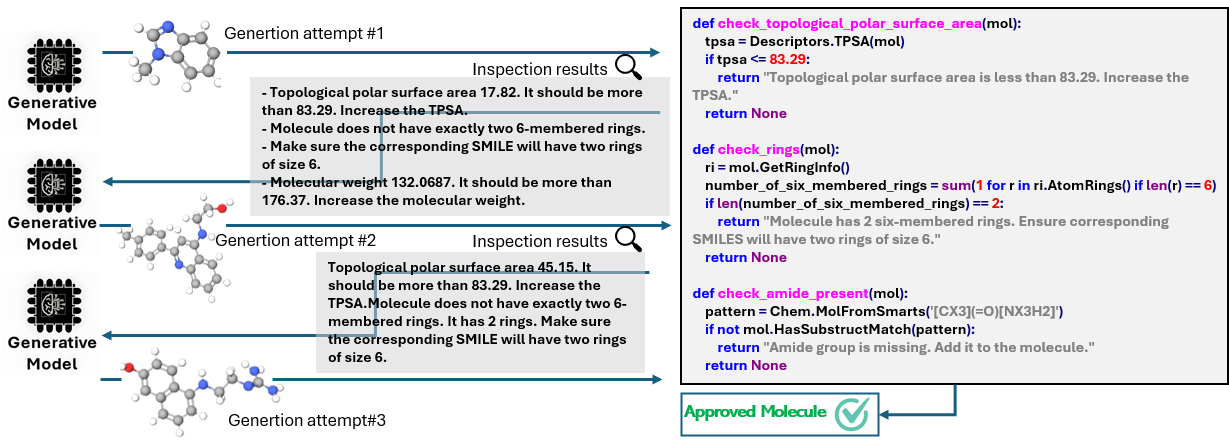
\includegraphics[width=0.8\linewidth]{figures/example.png}
        \caption{\small Overview of the CDMS iterative refinement approach for molecule generation. The left panel outlines the step-by-step process of refining molecular structures based on textual feedback, while the right panel demonstrates the Inspector model's generated code for validating molecular constraints. This code-driven feedback mechanism ensures alignment with user-defined requirements, enabling precise and iterative enhancements to the generated molecules.}
        \label{fig:mol_generation_feedback_example}
    \end{figure*}

% \textbf{(1)} We introduce a novel dataset that, unlike previous datasets which rely on a golden standard target molecule, provides NLP requirements coupled with an inspection mechanism capable of accepting any solution that satisfies the specified requirements.
% \textbf{(2)} We propose an iterative methodology that leverages an inspector model that uses code as an inspection tool to enhance generated output compliance. At each iteration, the inspector model evaluates the previous answer produced by the generative model using its specialized inspection code and provides text-based feedback with textual feedback to fix detected violations. Furthermore, we demonstrate how auto-evaluation using code achieves more accurate results regardless of the underlying generative model.
% \textbf{(3)} We present a novel approach to molecule discovery with wide-ranging applications in fields such as biology, including protein folding and beyond. This approach uses code to evaluate and provide precise, actionable feedback that aligns generative outputs more effectively with user requirements.

% \begin{figure}
%     \centering
%     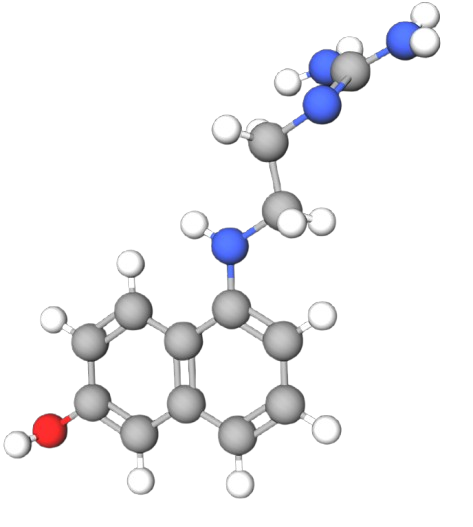
\includegraphics[width=0.5\linewidth]{figures/OC1_CC2_C_C_C1_C__CC_C2_NCCN_C_N_N-removebg-preview (1).png}
%     \label{fig:enter-label}
%     \noindent
%     \small
%     \begin{minipage}[t]{0.55\linewidth}
%         \textbf{Mol2Cap} \\
%             The molecule is a member of the class of hydroxyanthracenes that is 9 -hydroxyanthracene in which one of the hydrogens attached to the amino group has been replaced by a guanidino group. It is a member of guanidines, a member of phenols, an aromatic ether and a diphenylisochromene. It derives from a 9 -hydroxyanthracene.
%     \end{minipage}%
%     \hfill%
%     \begin{minipage}[t]{0.40\linewidth}
%         \textbf{ChemGen} \\
%             The molecule has a topological polar surface area exceeding 83.29, it contains an amine functional group, and it includes two rings, each consisting of six atoms. Additionally, the molecular weight is confined to a range between 176.37 and 450.34.
%     \end{minipage}
%     \caption{Proposed dataset CDMS against chEBI-20 dataset sample}
%     \label{fig:dataset_comparison}
% \end{figure}

    \lstset{
        language=Python,
        basicstyle=\ttfamily\small,
        keywordstyle=\color{blue},
        stringstyle=\color{red},
        commentstyle=\color{green},
        morecomment=[l][\color{magenta}]{\#},
        frame=single, % Add a frame around the code
        breaklines=true, % Wrap long lines
        numbers=left, % Line numbers on left
        numberstyle=\tiny\color{gray}, % Style of numbers
        showstringspaces=false % Don't show spaces in strings
    }


\section{Related work}

\textbf{Text-to-Molecule Generation.}  
Molecule synthesis from textual descriptions is a key area in molecular generation. Early work used SMILES (Simplified Molecular Input Line Entry System) representations — a textual format for encoding molecular structure- with BioT5+~\cite{pei-etal-2024-biot5} training a transformer on the ChEBI-20 dataset~\cite{edwards2021text2mol} that links molecular descriptions with structures.

Recent models have advanced alignment and generation strategies. MolReFlect~\cite{li2024molreflectincontextfinegrainedalignments} uses in-context alignment, and LDMol~\cite{chang2024ldmoltexttomoleculediffusionmodel} adopts a diffusion-based latent approach—though both lack public code. MoleculeSTM~\cite{liu2023moleculestm} enables text-guided molecule editing via contrastive learning in a joint latent space. More recently, mCLM~\cite{edwards2025mclmmodularchemicallanguage} proposes a modular chemical language model that represents molecules as synthesis-compatible functional building blocks aligned with natural language, enabling multimodal reasoning over molecular structure and function, but it fails to understand a complex set of constraints for molecule design as we show in Section~\ref{sec:main_results}.

LLM-based methods such as ChemLLM~\cite{zhang2024chemllm} and MolReGPT~\cite{molregpt} extend generation through domain specialization and retrieval-augmented generation, respectively. ChatDrug~\cite{liu2024chatdrug} and ChemCrow~\cite{bran2024chemcrow} introduce iterative loops using external tools like RDKit to guide improvements, but lack formal validation or enforcement of constraints.

In contrast, CDMS dynamically generates a single task-specific \emph{inspector} as executable code, which performs exhaustive, deterministic validation and returns \emph{Programmatic Feedback Gradients}. This enables an iterative refinement loop that continues until all constraints are satisfied—offering stronger compliance guarantees than retrieval- or tool-augmented methods.

\textbf{Iterative Refinement.}  
Iterative refinement is widely used in text generation, initially relying on human feedback~\cite{bai2022constitutional, fang2023single-step} and later on scalar rewards~\cite{Liu2022RainierRK} or free-form critiques~\cite{madaan2024self, shinn2023reflexion}. However, these methods struggle with complex, multi-constraint objectives.

Molecule optimization has followed similar trends, combining heuristics or expert-driven retrosynthesis~\cite{fang2023single-step, 10.1093/bioinformatics/btad157}, but these approaches lack scalability.

TextGrad~\cite{yuksekgonul2025optimizing} incorporates external tools to produce auxiliary validation signals and generates a new verification program at each iteration to evaluate the previous output. This design introduces additional call overhead and may lead to inconsistent inspection across iterations. The resulting signals are then interpreted by an LLM to determine the refinement strategy, while the enforcement of the inferred corrections is delegated to another LLM. 

In contrast, CDMS compiles task constraints into a persistent executable inspector (executable code) that deterministically verifies constraints and produces explicit corrective prompts as an output of the code directly, eliminating the need for LLM-based interpretation of validation signals at each iteration.
    
\section{CDMS Framework}
    \label{sec:cdms}
    In this section, we present CDMS—an iterative self-refinement methodology designed for the first phase of molecule synthesis, where candidate molecules are generated based on textual requirements. CDMS integrates code-enhanced feedback into the generation process, ensuring alignment with the specified constraints and improving the quality of the generated candidates.
    CDMS is composed of three distinct models: \textbf{(1)} the Memory component, which stores previous outputs and feedback; \textbf{(2)} the Generative Model ($M_G$), responsible for primary content generation; and \textbf{(3)} and the Inspector Model ($M_I$), which evaluates the generated content using generated code and provides approval or constructive feedback. We would like to emphasize that our model is versatile and can be applied to any generative model as $M_G$.
    In each iteration, \( M_G \) receives the input from both the user (i.e. the set of requirements) and the textual feedback provided by \( M_I \). Consequently, \( M_I \) takes the content generated by \( M_G \) to produce feedback for the next iteration of \( M_G \).
    We show that as long as the LLM understands the aspect to be optimized (e.g., reducing molecular weight translates to reducing molecule count or using lighter molecules) and there is a self-evaluation loop instructing which aspects to optimize, this can lead to more aligned molecules.
    This section details each component and how they function collaboratively within the CDMS framework.  
    We empirically show that CDMS outperforms previous SOTA models on ChemGen, a dataset we introduce, in addition to two synthetic tasks in natural language (NL) generation aimed to highlight LLM weak points that CDMS can help with.
        
    \subsection{Generative Model}
    The generative model can be any language model that supports a turn-by-turn input format. CDMS allows any model to be plugged in, where we show a performance boost in every model $M_G$. In our study, we experiment with foundation models with world knowledge and those designed for chemistry GPT-4.1~\cite{openai2025gpt41}, GPT-4o~\cite{openai2024gpt4technicalreport}, LLaMA3.3-70B~\cite{grattafiori2024llama3herdmodels}, and Claude3.5 Haiku~\cite{Anthropic2023}, while we also leverage more specialized models in the framework of CDMS, such as MolReGPT~\cite{molregpt}.

    \subsection{Inspector Model}
    \label{sec:inpector}
    The Inspector Model ($M_I$) is implemented as an NL-to-code generation system, specifically designed to generate code that evaluates whether a given SMILES representation of a molecule adheres to a set of constraints provided by the user in NL. The model is configured to decompose complex molecular requirements into smaller sub-requirements, enabling a fine-grained systematic evaluation of the molecule's compliance.

    The inspector generates the inspection code only once during the inference process, when obtaining user requirements. Unlike previous methods, this code can then be optionally reviewed by a human-in-the-loop and saved to $M_I$'s state and is reused at every iteration.
    At each iteration, $M_I$ inspects the SMILES formula against these requirements by executing the inspector code with the SMILES as a string input, identifying any violations, and producing \emph{programmatic actionable feedback} as seen in Figure~\ref{fig:mol_generation_feedback_example} for refinement. This iterative feedback mechanism is intended to ensure that the generated molecule progressively aligns with the specified constraints. Our implementation uses GPT-4o as the primary code generation backbone due to resource availability, with additional experiments utilizing alternative models detailed in Section~\ref{sec:code_generation_model}.

    

    \subsubsection{Code Generation and Execution}
    The model receives a prompt to generate Python code, i.e., the \emph{Inspector code}, that checks whether a given set of constraints is satisfied. If a constraint is not met, the generated code function should return a list of textual feedback describing the violation and the necessary modifications for each violation.
    
    The generated code follows a format where 
    each constraint is implemented as a single method, ensuring modularity and clarity. A single entry point orchestrator function is responsible for running these inspector methods and returning aggregated results, maintaining consistency, and reducing variability. For reproducibility and further exploration, we provide the prompt used in Appendix~\ref{app:model_prompts}.


    \subsubsection{Feedback Generation}
    The code generation model is instructed to generate an entry point method that encapsulates other method calls. CDMS invokes the entry point method with the generated molecule SMILES and receives the list of feedback, then compiles it back to a textual format to be passed to $M_G$.

    \subsubsection{Enhancing Code Reliability}
    \label{sec:enhancing_code_stability}

    To minimize the variability of the generated code and improve precision, the code generation model is supplied once with a single targeted few-shot example. This example is an illustration of what we expect the code to do and how to structure it.
    % The generated code follows a format where each constraint is implemented as a single method, ensuring modularity and clarity. A single entry point orchestrator function is responsible for running these inspector methods and returning aggregated results, maintaining consistency, and reducing variability.
    
    We draw the reader's attention to the fact that this example is supplied to the code generation model as a few-shot and is not tailored per task. This example is important in guiding the code generation process, ensuring that the generated code structure reflects intended functions and conforms to required formats with less reliance on extensive prompt engineering. Given these measures and considering the clear, easy-to-read textual format of the input, we did not observe significant instances of inaccurate code that justify further action.
    
% \subsubsection{Code Alignment with Requirements}
% We use prompt engineering with few-shot prompting to tune the code generation model for task-specific code generation. The problem of alignment between NLP and the generated code is not solved in the field of code generation~\cite{uniyal-etal-2024-one}, we also do not propose an algorithmic framework to ensure alignment, yet we empirically show that with our method we achieve a performance boost of (30\%-60\%). We manually evaluate the alignment of the code, please see Section~\ref{sec:code_alignment}

    \subsection{Memory}
    \label{sec:memory}
    The memory component is essential for preserving the context of interactions between the generative model and the inspector model. It serves as a dynamic log, recording each attempt by the generative model and the corresponding feedback from the inspector. This log links all prior interactions, allowing the generative model to reference and learn from past failures, similar to revisiting an advisor's feedback. The generative model uses this memory as input, we use the memory as in-context learning to prevent the generative model from repeating previous mistakes. The data in this memory is organized in JSON format as seen in Figure~\ref{fig:memory_structure} %detailed information about this structure is available in Appendix~\ref{sec:memeory_format}.

\begin{figure}[h]
    \begin{minipage}{0.95\linewidth}
    \small
    \texttt{[}\\
    \texttt{\ \ \{"role": "user", "content": "<task specification>"\},}\\
    \texttt{\ \ \{"role": "assistant", "content": "<candidate output>"\},}\\
    \texttt{\ \ \{"role": "user", "content": "<inspector feedback>"\},}\\
    \texttt{\ \ \{"role": "assistant", "content": "<revised candidate output>"\}}\\
    $\dots$\\
    \texttt{]}
    \end{minipage}
\caption{Structure of the memory buffer that records generator outputs and inspector feedback during iterative refinement.}    \label{fig:memory_structure}
\end{figure}


    % We log every generation–inspection exchange. This in-context record lets the generator review past feedback and avoid repeating earlier errors (more details can be found in Appendix \ref{sec:memeory_format}).
    

    \subsection{Iterative Algorithm}

    The generation process is outlined in Algorithm~\ref{alg:generation_process}. The inspector and generator arrangement establishes an adversarial yet constructive feedback loop. In this loop, the interaction is akin to a dialogue from the perspective of the generative model, which retains the memory of previous exchanges. This memory aids the generative model in avoiding past mistakes and preventing the repetition of errors. The code generation model, on the other hand, is specifically tuned to the numerical and structural attributes of the text. It generates feedback that the generative model uses to refine its outputs. This dynamic ensures that the generated content is not only accurate but also contextually relevant.

    \begin{algorithm}
        \caption{CDMS algorithm}
        \label{alg:generation_process}
        \begin{algorithmic}[1]
            \STATE \textbf{Input:} NLP molecule requirements.
            \STATE \textbf{Output:} Content adheres to the constraint.
            \STATE
            \STATE inspector\_code $\leftarrow$ Inspector(constraints)
            \STATE feedback $\leftarrow$ constraint
            \STATE attempt count $n \leftarrow 0$
            \WHILE{$n <$ maximum optimization attempts}
            \STATE response $\leftarrow$ GenModel(feedback)
            \STATE feedback $\leftarrow$ inspector\_code.exec(response)
            \IF{feedback is approval}
            \RETURN approved content
            \ENDIF
            \STATE $n \leftarrow n + 1$
            \ENDWHILE
            \RETURN response
        \end{algorithmic}
    \end{algorithm}

    Please note that upon exceeding the maximum number of optimization attempts, CDMS outputs the last molecule generated, together with a signal if the inspector approves it.

    
\section{Empirical Evaluation}
    In this section, we present the empirical evaluation framework, along with the baselines, datasets, and methods used to assess our model.

    \subsection{Datasets}
    \label{sec:dataset}

Datasets in de novo molecule generation such as Text2Mol~\cite{edwards2021text2mol} and LlaSMol~\cite{yu2024llasmol} typically define a single ``golden'' target molecule because the natural language description specifies a single exact molecular structure. In contrast, our setting describes a \emph{set of constraints} that a valid molecule must satisfy. For a given set of attributes, many molecules may satisfy the requirements. Consequently, datasets designed for single-target reconstruction are not suitable for evaluating constraint-driven molecule generation. To address this limitation we introduce \textbf{ChemGen}, a dataset for generating molecules from natural language requirements expressed as sets of molecular constraints.

ChemGen adopts a one-to-many evaluation paradigm: multiple molecules may satisfy the same requirement set. Instead of comparing generated molecules to a single ground-truth structure, evaluation verifies whether the generated molecule satisfies all constraints. To enable this evaluation, each requirement is paired with an expert-authored executable \textit{validation program} (``golden code'') that deterministically checks constraint satisfaction.

\subsection{Dataset Construction}

The dataset was constructed through collaboration between chemists and computer scientists. Chemists curated a diverse collection of molecular properties commonly studied in chemical compound databases such as PubChem~\cite{kim2023pubchem}. These include physicochemical attributes (e.g., molecular weight and topological polar surface area), structural properties (e.g., ring counts and rotatable bonds), and functional group requirements describing chemical reactivity.

Computer scientists implemented executable validators for each requirement using code-based routines that compute molecular descriptors and verify constraint satisfaction. For every requirement set, chemists identified at least one molecule from PubChem satisfying the constraints, ensuring that each entry corresponds to a chemically realizable compound.

Natural language requirements follow a structured constraint language that combines molecular properties, comparison operators, and functional group patterns.

\subsection{Dataset Statistics}

ChemGen contains 779 unique samples and a total of 4,599 constraints. Each compound is associated with a set of 3--9 requirements (5.9 on average), reflecting the constraint-driven formulation of the task. 

The constraints span multiple molecular property categories and comparison operators. In total, the dataset includes molecular properties, such as ring counts, covalent bond counts, molecular weight, topological polar surface area (TPSA), heavy atom counts, rotatable bonds, and functional group requirements. These properties are expressed through ten comparison operator types (e.g., inequalities, bounded ranges, equality relations, and presence or absence constraints). Across the dataset, the natural language descriptions are generated from 53 unique requirement templates (after abstracting numerical values), and functional group detection is implemented using 18 SMARTS patterns corresponding to chemically meaningful substructures. This structure allows ChemGen to represent a diverse range of molecular requirements while maintaining consistent evaluation through executable validation code.

Finally, we analyze how restrictive the constraint sets are by measuring how many molecules in PubChem satisfy the specified requirements. PubChem currently contains approximately 115 million compounds, providing a large reference space for evaluating constraint difficulty.  For many entries in ChemGen, the requirements narrow this space to only a small number of candidates. In 0.4\% of the dataset, only one molecule in the entire PubChem database is expected to satisfy the constraints, indicating extremely restrictive requirement sets. Only 8.4\% of entries correspond to more than 1,000 candidate molecules in PubChem, despite the database containing over 115 million compounds. Overall, these statistics demonstrate that ChemGen does not consist of trivial constraint descriptions: many requirement sets isolate only a very small fraction of the molecules in a database of more than 115 million compounds, making the generation task significantly constrained.

% We present a novel dataset for NL-requirements-to-molecule generation, addressing the challenge of translating textual specifications into valid molecular structures. Chemists curated a diverse set of sought-after features in molecules that are studied and annotated in chemical compound corpuses such as Pubchem~\cite{kim2023pubchem}. We then composed a dataset of 779 entries that have a subset of these requirements. These requirements include solubility, which indicates how well a compound dissolves; surface area, which can be beneficial if we want to create another molecule from it; and functional groups, which indicate reactivity with other materials, among others. Computer scientists annotated each requirement with executable code snippets designed to verify molecular compliance. Chemists then proposed at least one molecule from PubChem~\cite{kim2023pubchem} that satisfies the given requirements set to ensure these requirements can be met by a real molecule.

% Unlike existing text-to-molecule datasets~\cite{edwards2021text2mol}, which focus on generating a single "gold standard" molecule, our dataset acknowledges the possibility of multiple valid molecules satisfying the same set of requirements. To accommodate this flexibility, each requirement is paired with \textit{"golden"}-validation code to ensure the evaluation of each constraint in the generated molecule. This approach supports robust benchmarking and facilitates advancements in molecule generation research. Examples from our dataset can be found in Appendix~\ref{sec:dataset_samples}.

    \subsection{Baselines}
    \label{sec:baselines}
    We evaluate CDMS  against several baselines, including zero-shot generative models, iterative refinement models, and task-specific trained models.
    We use GPT-4.1, GPT-4o, LLaMA-3.3-70b, and Claude 3.5 for the underlying generative models. Additionally, we experiment with advanced prompt engineering techniques, such as chain-of-thought reasoning and few-shot generation, to enhance performance by structuring tasks more effectively and providing examples for context.

    For iterative refinement, we select Self-Refine~\cite{madaan2024self}, which employs iterative refinement with textual self-feedback generated by the LLM to progressively improve model outputs. We additionally evaluated TextGrad~\cite{yuksekgonul2025optimizing}, which incorporates external tools such as RDKit~\cite{rdkit} in an iterative, tool-guided generation setup. However, the original TextGrad work does not report empirical results on molecule generation performance at all so we benchmark it on ChemGen. For a fair comparison, we adapted the CDMS feedback prompt to TextGrad’s input format. Both TextGrad and Self-Refine were allowed the same number of refinement iterations during evaluation. Notably, access to code or chemistry tools is not unique to CDMS: TextGrad also uses executable code and external tools such as RDKit.

    We benchmark specialized models: ChemLLM~\cite{zhang2024chemllm} as an LLM dedicated to chemistry and trained on molecule generation, and mCLM~\cite{edwards2025mclmmodularchemicallanguage}, a modular chemical language model that jointly models natural language and molecular structures by representing molecules as synthesis-aware functional building blocks rather than atom-level tokens.

    We finetuned BioT5+~\cite{pei2024biot5+}, a model trained on the ChEBI-20~\cite{Shardlow2018} and considered SOTA on Text2Mol dataset~\cite{edwards2021text2mol} for text-to-molecule tasks. Appendix~\ref{app:baseline_finetuning} provides more details about the fine-tuning process. we draw the reader’s attention to the fact that ChemGen does not have an aligned golden-standard molecule that intuitively supports fine-tuning, but used the ChemGen raw data (see Section~\ref{sec:dataset}).

% We also include MolReGPT~\cite{molregpt}, a specialized model leveraging a foundational architecture, as another strong baseline for molecule generation tasks. and supply relevant samples to MolReGPT from our own dataset to tune it to the task specific.
    We also include MolReGPT~\cite{molregpt}, the SOTA generative model designed to create molecular structures based on textual descriptions. In the analysis below, we refer to it as MolRe-$X$ for generality.

    To demonstrate the versatility of CDMS as a framework compatible with various models, we incorporate CDMS using MolReGPT as the underlying generative model.

    We use GPT-4.1, GPT-4o, LLaMA-3.3-70B, and Claude 3.5 Haiku as the main generator backbones in our experiments. Later we refer to CDMS as the configuration with CDMS frameworks leveraging MolReGPT with GPT-4o as its generative backbone.

    Some specialized molecule generation models (e.g., mCLM, ChemLLM, BioT5+) are evaluated only in a standalone setting. These models do not support multi-turn or feedback-conditioned generation, and therefore cannot be integrated into the CDMS refinement loop.
    
    \subsection{Metrics and Evaluation}
    We evaluate the performance of CDMS and baseline models (see Section~\ref{sec:baselines}) on our custom dataset (see Section~\ref{sec:dataset}). The evaluation metric is the percentage of outputs generated by each model that comply with the specified molecular requirements.

    
\section{Empirical Results}
    % In this section, we discuss our empirical findings and ablation studies. We explore the individual contributions of each component to overall performance, specifically examining the impact of both the coder and text generation models on the performance of CDMS.

    \subsection{Main Result}
    \label{sec:main_results}
\begin{table*}[h!]
    \centering
    \small
    \begin{tabular}{llp{1.5cm}p{1.5cm}p{1.5cm}p{1.5cm}}
        \toprule
        \textbf{Category} & \textbf{Framework} & \textbf{GPT-4.1} & \textbf{GPT-4o}  & \textbf{LLaMA-3} & \textbf{Claude 3.5} \\
        \midrule
        \textbf{LLM Prompting Strategies}
        & Zero-Shot                        & 36.30            & 25.42            & 22.72            & $7.06$             \\
        & Chain-of-Thought (CoT)           & 31.10            & 29.41            & 37.25            & $12.58$            \\
        & Few-shot                         & 32.60            & 28.23            & 36.17            & $13.09$            \\
        & CoT + Few-shot                   & 37.08            & 30.84            & 39.01            & $16.17$            \\
        \midrule
        \multirow{3}{*}{\textbf{Molecular Design Strategy}}
        & MolRe-$X$~\cite{molregpt}        & 38.20            & 43.13            & 35.49            & 23.62              \\
        & \cellcolor{gray!20} ChemLLM~\cite{zhang2024chemllm}& \multicolumn{4}{c}{\cellcolor{gray!20}------------ 5.59 (standalone) ------------} \\& \cellcolor{gray!20} mCLM~\cite{zhang2024chemllm}& \multicolumn{4}{c}{\cellcolor{gray!20}------------ 3.9 (standalone) ------------} \\
        \midrule
        \multirow{3}{*}{\textbf{Iterative Feedback}}
        & Self-Refine~\cite{madaan2024self} & 60.0               & $26.83$          & $24.39$          & $15.01$            \\
        & TextGrad~\cite{yuksekgonul2025optimizing} & 61.3 & $25.83$ & $28.17$ & $21.13$\\
        & k-attempts ($k=7$) & 37.0 & $26.24$ & $23.82$ & $7.19$ \\        \midrule
        \textbf{Finetuned model} 
        & \cellcolor{gray!20} BioT5+
        & \multicolumn{4}{c}{\cellcolor{gray!20}------------ 25.93 (standalone) ------------} \\
        \midrule
        \multirow{5}{*}{\textbf{CDMS}}
        & Zero-Shot                        & $63.10$ & $35.30$          & $34.19$          & $23.74$            \\
        & CoT$^*$                          & $64.81$ & $39.15$          & $52.94$          & $24.00$            \\
        & Few-shot                         & $72.67$ & $41.91$          & $48.00$          & $24.18$            \\
        & CoT + Few-shot                  & $83.70$ & $48.09$          & $53.92$          & $25.80$            \\
        & MolRe-$X$                        & $\textbf{86.35}$ & $\textbf{51.47}$ & $\textbf{54.34}$   & $\textbf{35.04}$    \\
        \bottomrule
    \end{tabular}

    \caption{Performance of models with different optimization approaches. Grayed rows indicate standalone results that do not rely on LLMs. * Generator and inspector models both use CoT }
    \label{tab:model_results}
\end{table*}

Table~\ref{tab:model_results} presents a comparative analysis of task-expert models, baseline LLMs and numerous prompting and refinement approaches.
In this experiment, for a given set of textual constraints, the baselines were tasked with generating a molecule that adheres to chemical requirements. Results in bold show the winner in each model column, and all results in bold are statistically significant\footnote{Statistical significance was assessed for all baselines using McNemar’s test on paired binary outcomes ($\alpha = 0.05$); results were deemed significant when $p < 0.05$}.

We observe that GPT-4.1 is the strongest GPT-based model and achieves particularly high performance under iterative feedback strategies. LLaMA-3 generally outperforms GPT-4o and Claude 3.5 in standard prompting settings, especially in methods like Chain-of-Thought (CoT) and CoT + Few-shot. MolRe-X, a molecular design model, provides a strong specialized baseline, as expected from a task-specific model.

The CDMS strategy consistently delivers the best results, regardless of the baseline model used (GPT-4.1, GPT-4o, LLaMA-3, or Claude 3.5) or the prompting strategy. Notably, MolRe-X also achieves its highest performance under the CDMS strategy, demonstrating its effectiveness in molecular design tasks. This trend holds for all models tested, where the iterative textual feedback improves upon any optimization strategy. 

We observed that an LLM with k-attempts, where multiple outputs are generated simultaneously without interconnection, yields lower results compared to CDMS. This highlights the importance of the feedback mechanism, as opposed to relying solely on multiple iterations.
We also observe the superiority of our model compared to other textual feedback models that are not based on code, such as Self-Refine.
Additionally, we experimented with fine-tuned BioT5+, which achieved a non-trivial standalone result. However, its reliance on a large amount of annotated and aligned data raises concerns about its scalability.

Importantly, code-based feedback is not unique to CDMS: TextGrad also generates and executes validation code during refinement. CDMS nevertheless consistently outperforms TextGrad, indicating that its gains are not merely a consequence of using code in a benchmark evaluated with executable validators. Moreover, TextGrad generates a new verification program at every iteration, producing substantially more code overall, yet still underperforms CDMS, which relies on a single persistent inspector reused throughout refinement.

% \subsection{Main Result}
% \label{sec:main_results}
    
% \begin{table*}[h]
% \centering
% \small
% \begin{tabular}{l l c c c c}
% \toprule
% \textbf{Baseline} & \textbf{Method} & \textbf{GPT-4.1} & \textbf{GPT-4o} & \textbf{LLaMA-3} & \textbf{Claude 3.5} \\
% \midrule

% \multirow{2}{*}{Zero-Shot}
% & Baseline & 36.3 & 25.42 & 22.72 & 7.06 \\
% & +CDMS & \textbf{63.10} & \textbf{35.30} & \textbf{34.19} & \textbf{23.74} \\

% \midrule

% \multirow{2}{*}{Chain-of-Thought}
% & Baseline & 31.1 & 29.41 & 37.25 & 12.58 \\
% & +CDMS & \textbf{64.81} & \textbf{39.15} & \textbf{52.94} & \textbf{24.00} \\

% \midrule

% \multirow{2}{*}{Few-Shot}
% & Baseline & 32.6 & 28.23 & 36.17 & 13.09 \\
% & +CDMS & \textbf{72.67} & \textbf{41.91} & \textbf{48.00} & \textbf{24.18} \\

% \midrule

% \multirow{2}{*}{CoT + Few-Shot}
% & Baseline & 37.08 & 30.84 & 39.01 & 16.17 \\
% & +CDMS & \textbf{83.70} & \textbf{48.09} & \textbf{53.92} & \textbf{25.80} \\

% \midrule

% \multirow{2}{*}{MolRe-X}
% & Baseline & 38.2 & 33.13 & 35.49 & 23.62 \\
% & +CDMS & \textbf{86.35} & \textbf{51.47} & \textbf{54.34} & \textbf{35.04} \\

% \midrule
% \multicolumn{2}{c}{\textbf{Standalone Models}} & & & & \\
% \midrule
% \multirow{3}{*}{Specialized Models}
% &mCLM &\multicolumn{4}{c}{------ \qquad 3.9 \qquad ------}\\
% &ChemLLM &\multicolumn{4}{c}{------ \qquad 5.6 \qquad ------}\\
% &Fine-Tuned BioT5+ &\multicolumn{4}{c}{------ \qquad 25.93 \quad ------}\\
% \bottomrule
% \end{tabular}

% \caption{\small Performance on the ChemGen constraint-driven molecule generation task. We report the percentage of generated molecules that satisfy all textual constraints. Each baseline prompting strategy or molecular design model is evaluated both independently and when integrated with the CDMS framework if its archeticture allows it. CDMS consistently improves constraint satisfaction across all prompting configurations and backbone models. For specialized models (mCLM, ChemLLM, BioT5+), results correspond to standalone performance as these systems are not compatible with the CDMS refinement loop.}
% \label{tab:cdms_vs_baselines}
% \end{table*}

% \begin{table}[h]
% \centering
% \small
% \begin{tabular}{l c c c c}
% \toprule
% \textbf{Method} & \textbf{GPT-4.1} & \textbf{GPT-4o} & \textbf{LLaMA-3} & \textbf{Claude 3.5} \\
% \midrule
% Zero Shot & 36.3 & 25.42 & 22.72 & 7.06 \\
% k-attempts ($k=7$) & 37.0 & 26.24 & 23.82 & 7.19 \\
% Self-Refine & 60.0 & 26.83 & 24.39 & 15.01 \\
% TextGrad & 61.3 & 25.83 & 28.17 & 21.13 \\
% \midrule
% \rowcolor{lightgray} ZeroShot + CDMS & \textbf{63.10} & \textbf{35.30} & \textbf{34.19} & \textbf{23.74} \\
% \bottomrule
% \end{tabular}

% \caption{\small Comparison with iterative refinement baselines on the ChemGen constraint-driven molecule generation benchmark. Results report the percentage of generated molecules that satisfy all specified constraints. We compare standard prompting (Zero-Shot), repeated sampling without feedback (k-attempts), and existing iterative refinement methods (Self-Refine and TextGrad). The final row shows the performance of CDMS applied to the same zero-shot generation setting, demonstrating that static executable constraint validation provides stronger improvements than purely textual feedback or repeated sampling.}
% \label{tab:iterative_refinement}
% \end{table}

%     % Table~\ref{tab:model_results} presents a comparative analysis of task-expert models, baseline LLMs, and multiple prompting and refinement approaches.

%     % In this experiment, for a given set of textual constraints, the baselines were tasked with generating a molecule that adheres to chemical requirements. Results in bold indicate the best-performing method for a given mdoel. All bolded results are statistically significant\footnote{Statistical significance was assessed for all baselines using McNemar’s test on paired binary outcomes ($\alpha = 0.05$); results were deemed significant when $p < 0.05$}.
    
%     % Among the baseline language models, GPT-4.1 achieves the strongest performance overall. In standard prompting settings (Zero-Shot, Few-shot, and CoT + Few-shot), GPT-4.1 consistently outperforms GPT-4o, LLaMA-3, and Claude 3.5. LLaMA-3 remains competitive in several prompting configurations, particularly under Chain-of-Thought prompting, while Claude 3.5 generally achieves the lowest results across these baselines.
    
%     % MolReGPT, a specialized molecular design model, achieves strong performance relative to general-purpose LLM prompting strategies, which is expected given its domain specialization. However, its results are still substantially improved when combined with the CDMS framework.
    
%     % Across all baseline models (GPT-4.1, GPT-4o, LLaMA-3, and Claude 3.5), the CDMS strategy consistently yields the strongest results regardless of the prompting configuration. Notably, MolRe-X (MolRe-GPT with a substituted generative model) also achieves its highest performance when combined with CDMS, suggesting that the iterative constraint verification mechanism improves performance even for specialized molecular design systems. This pattern holds consistently across all evaluated models, where iterative feedback enables systematic correction of constraint violations.
    
%     % We further observe that a k-attempt generation strategy, where multiple candidate molecules are generated independently without interaction or feedback, produces weaker results compared to CDMS. This result highlights the importance of the feedback mechanism rather than relying solely on repeated sampling.
    
%     % CDMS also outperforms alternative textual feedback approaches that do not incorporate executable verification, such as Self-Refine. While TextGrad generates code at every iteration and is therefore computationally more intensive, CDMS achieves stronger performance using a single inspector combined with an executable textual gradient.
    
%     % Finally, we evaluated the fine-tuned BioT5+ model, which achieves competitive results. However, this approach requires large amounts of annotated and aligned training data, raising questions about scalability and data efficiency.

%     % In the following sections, CDMS refers to the CDMS framework implemented with MolReGPT and GPT-4o as the generative model.    
% % -----
% % Tables~\ref{tab:cdms_vs_baselines} and~\ref{tab:iterative_refinement} summarize the main results on the ChemGen constraint-driven molecule generation benchmark. We report the percentage of generated molecules that satisfy all textual constraints. In Table~\ref{tab:cdms_vs_baselines}, each prompting strategy or molecular design baseline is evaluated both on its own and when augmented with CDMS. Table~\ref{tab:iterative_refinement} focuses on iterative refinement baselines and compares CDMS against repeated sampling and iterative-refinement-based methods. Bold results denote the best result for each backbone model, and all bolded improvements are statistically significant.\footnote{Statistical significance was assessed using McNemar’s test on paired binary outcomes with $\alpha = 0.05$; improvements are considered significant when $p < 0.05$.}

% % Among the standalone prompting baselines seen in Table~\ref{tab:cdms_vs_baselines}, GPT-4.1 is the strongest general-purpose model overall, and it is reflected in its zero-hot performance on ChemGen: it achieves the best performance under Zero-Shot, Few-Shot, and CoT + Few-Shot prompting, while LLaMA-3 is particularly competitive under Chain-of-Thought prompting. Claude 3.5 consistently underperforms the other backbones in these standard prompting settings. The specialized molecular design baseline MolRe-X is stronger than most vanilla prompting strategies, which is expected given its domain-specific design, but it still leaves substantial room for improvement under strict multi-constraint generation.

% % Across all prompting configurations and backbone models, augmenting generation with CDMS yields the strongest results. This trend is highly consistent: Zero-Shot + CDMS improves over Zero-Shot for every backbone, and the same holds for Chain-of-Thought, Few-Shot, CoT + Few-Shot, and MolRe-X. For example, GPT-4.1 improves from 36.3 to 63.10 under Zero-Shot, from 32.6 to 72.67 under Few-Shot, and from 38.2 to 86.35 when MolRe-X is combined with CDMS. Similar improvements appear for GPT-4o, LLaMA-3, and Claude 3.5, indicating that the benefit of CDMS does not depend on a particular model family or prompting style.

% % These improvements support the central claim of CDMS: performance benefits from shifting constraint checking and feedback generation away from free-form LLM reasoning and into a static executable inspector. CDMS uses a single verified code artifact that comprehensively evaluates the user constraints and is reused across all refinement iterations. This makes the refinement process stable and programmatic: at each step, feedback is generated by executing the inspector on the current candidate molecule, rather than asking the language model to infer on its own what failed and how to repair it. In other words, the burden of constraint reasoning is substantially reduced because violation detection is performed explicitly in code.

% % Table~\ref{tab:iterative_refinement} further clarifies this point. Repeated sampling alone is not enough: $k$-attempts yields only minor improvements over Zero-Shot, showing that simply generating more candidates without structured correction is weak. Self-Refine performs better than repeated sampling for some models, but it still relies on textual self-critique produced by the model itself, which makes the quality of refinement dependent on the model’s ability to correctly diagnose its own mistakes. TextGrad improves further, but its refinement loop constructs new code during the optimization process, making it both more computationally involved and less stable across iterations.

% % CDMS outperforms these alternatives by using a different refinement principle. Instead of regenerating the reasoning scaffold at each step, it keeps the inspector fixed and verified, and derives feedback directly from execution. This distinction matters: the model is not asked to repeatedly rediscover the constraint logic, and the feedback does not depend on whether the LLM can reliably explain its own failure modes. As a result, Zero-Shot + CDMS surpasses Zero-Shot, $k$-attempts, Self-Refine, and TextGrad across all evaluated backbones, showing that executable, persistent verification is more effective than repeated sampling or purely textual refinement.

% % We also report three specialized standalone models that are not suitable for integration into the CDMS refinement loop: mCLM, ChemLLM, and fine-tuned BioT5+. Their results provide additional context for the difficulty of the task. While fine-tuned BioT5+ achieves competitive standalone performance, it depends on dedicated supervised training and aligned data that are not available without serious investment in data collection, unlike CDMS, which improves a range of backbone generators without requiring task-specific fine-tuning. The inability to directly embed these models into the iterative CDMS loop also highlights an important practical distinction between specialized end-to-end systems and a modular refinement framework based on executable verification.

% % Unless stated otherwise, in the following sections CDMS refers to the full CDMS framework with an executable inspector and iterative refinement loop, instantiated with the relevant backbone generator for each experiment.

% Tables~\ref{tab:cdms_vs_baselines} and~\ref{tab:iterative_refinement} summarize the main results on the ChemGen constraint-driven molecule generation benchmark. In this experiment, for a given set of textual constraints, the baselines were tasked with generating a molecule that satisfies the specified chemical requirements. Results in bold indicate the best-performing method for a given model. All bolded results are statistically significant.\footnote{Statistical significance was assessed for all baselines using McNemar’s test on paired binary outcomes ($\alpha = 0.05$); results were deemed significant when $p < 0.05$.}

% Table~\ref{tab:cdms_vs_baselines} presents a comparative analysis of CDMS-compatible generative approaches: standard prompting baselines, MolReGPT: a specialized molecular design baseline, and their corresponding variants augmented with CDMS. Among the standalone language model baselines, GPT-4.1 achieves the strongest overall performance. In standard prompting settings, it consistently outperforms GPT-4o, LLaMA-3, and Claude 3.5, while LLaMA-3 remains competitive under Chain-of-Thought prompting. Claude 3.5 generally achieves the weakest results across these baselines. MolRe-X, a specialized molecular design model, performs strongly relative to general-purpose prompting strategies, which is expected given its domain specialization. However, its performance is also substantially improved when combined with CDMS.

% Across all evaluated backbones and prompting settings in Table~\ref{tab:cdms_vs_baselines}, CDMS consistently yields the strongest results. This includes both general-purpose prompting strategies and the specialized MolRe-X baseline, whose best performance is also obtained when paired with CDMS. These results support our hypothesis that molecule generation benefits from a refinement process grounded in explicit constraint verification. Rather than relying on the model alone to implicitly track which constraints were violated, CDMS applies a static verified inspector throughout the refinement loop, enabling systematic detection and correction of failures across iterations.

% Table~\ref{tab:iterative_refinement} focuses on iterative refinement baselines and clarifies the distinction between improvement due to repeated attempts and improvement due to executable feedback. The Zero-Shot and $k$-attempt baselines test whether stronger performance can be obtained simply by sampling more candidates without feedback. Their weaker results suggest that repeated generation alone is insufficient. Self-Refine introduces iterative textual feedback, but still places the burden of diagnosing failures on the language model itself leading to an improved performance over the zero-shot LLM. TextGrad also performs iterative refinement using code, but generates new code at each iteration, making the optimization process more computationally intensive and dependent on repeatedly reconstructed reasoning. Unlike CDMS, TextGrad delegates the understanding and reasoning over the code-generated signals onto the LLM, the LLM decides what action to take, unlike CDMS that generates this output in the code itself, allowing the LLM to focus on the improvement with explicit and reliable instructions.

% CDMS uses a single comprehensive inspector that is generated once, verified, and then reused across all iterations. The feedback is produced programmatically by executing this inspector, rather than by asking the language model to reason about its own errors in free text. The results in Table~\ref{tab:iterative_refinement} suggest that this distinction is important: CDMS outperforms repeated sampling and alternative refinement methods, supporting our central hypothesis that persistent executable verification provides a stronger and more reliable refinement signal than either unguided repetition or purely textual self-correction.

% Finally, we report the performance of several specialized standalone models that are not suitable for integration into the CDMS refinement loop, including mCLM, ChemLLM, and fine-tuned BioT5+. These results provide additional context for the difficulty of the task. While fine-tuned BioT5+ achieves competitive standalone performance, it requires aligned training data and task-specific supervision, raising questions about scalability and data efficiency relative to CDMS.

%     In the following sections, CDMS refers to the CDMS framework implemented with MolRe-X and GPT-4o as the generative model.
    
    \subsection{Number of Refinement Attempts}
    We analyzed the intermediate outputs of CDMS with GPT-4o to determine the percentage of results, whether accepted or rejected by the inspector, that are validated by the golden validator. The results, presented in Figure~\ref{fig:iterative_improvement}, highlight the performance of the two generator backbones analyzed in this refinement-depth study, GPT-4o and LLaMA-3. We demonstrate that the quality of results improves as the number of refinement iterations increases, with optimal performance at 7 attempts. This analysis over a separate validation set was also instrumental in tuning the hyperparameter for the number of refinement iterations. We draw the reader's attention that these are not the performance results of CDMS but the intermediate results that are yet to be accepted or rejected by the inspector model.

    \begin{figure}[h]
        \centering
        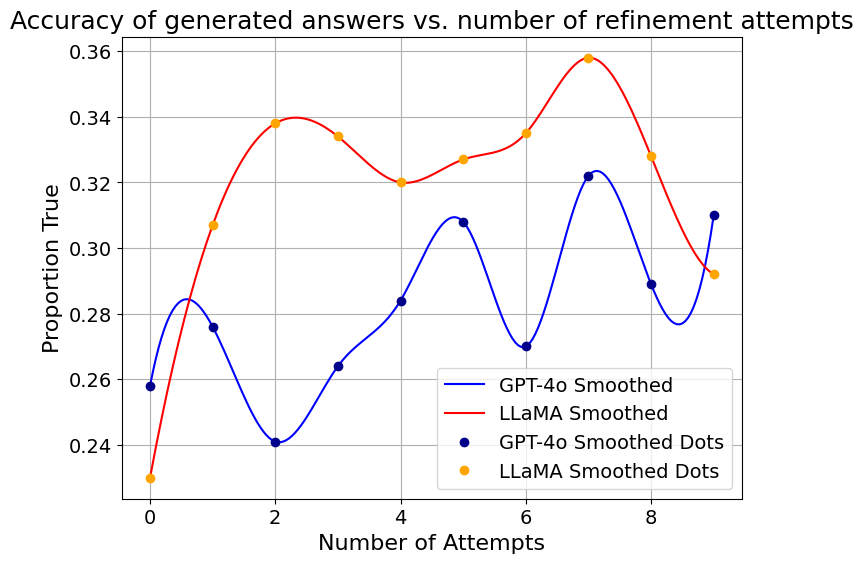
\includegraphics[width=0.5\linewidth]{figures/accuracy_vs_attempts.png}
        \caption{\small CDMS quality results in improvement vs. refinement attempts \emph{not} including the last iteration result approved by the inspector. Note that these results are lower than CDMS's performance results, as they include generation attempts unapproved by the inspector as well.}
        \label{fig:iterative_improvement}
    \end{figure}

    \subsection{Molecular Novelty and Diversity}
    We compared our generated results with the PubChem molecule dataset~\cite{kim2023pubchem} and found that 73.77\% of the generated molecules were not present in the dataset, demonstrating that CDMS acts as a molecule generator rather than merely retrieving known compounds, highlighting its potential in drug discovery. In addition, we analyzed the structural variation among the generated molecules and found an average molecular diversity (Tanimoto-based) of 0.898, compared to 0.903 for the original molecules from which the ChemGen dataset was constructed. This indicates that CDMS maintains a high level of chemical diversity while satisfying complex constraints.

    \subsection{Inspector Quality}

    In this ablation, we vary only the inspector-generation model, while keeping the generator fixed (GPT-4o). To evaluate the impact of the inspector component's coder model in CDMS, we perform an ablation study using generative models known to produce lower-quality code. As shown in Figure~\ref{fig:inspector_quality_ablation}, the overall accuracy of CDMS degrades with weaker models. Notably, even when using GPT-4o mini—which demonstrates poor performance on the SWE-benchmark~\cite{jimenez2024swebench}—CDMS maintains competitive performance. In fact, CDMS with GPT-4o mini slightly underperforms MolReGPT, the next best model, despite relying on a substantially weaker code generator.

    \subsection{Ablation Tests}
    \label{sec:ablation_tests}

    To evaluate the effectiveness of each component in our framework, we conducted the following ablation tests. For ablations that isolate a single component, we fix the generator to GPT-4o to maintain comparability with the original experimental setup and vary only the component under study.

    \subsubsection{Binary vs. Text Feedback}
    We aim to test the type of code used to generate feedback. Specifically, we will evaluate the impact of codes that generate textual feedback versus those that produce simpler binary inspectors, which return a binary signal based on whether the inspector approves or rejects the proposed molecule. We ran the experiment with two representative high-performing backbones from the original ablation setting. The results presented in Table~\ref{tab:binary_feedback} clearly show the effectiveness of the textual feedback in CDMS.

\begin{table}[h]
    \centering
    \small % Reduce font size to ensure it fits in a single column
    \begin{tabular}{l | ll | ll}
        \toprule
        \textbf{Methodology} & \multicolumn{2}{c|}{\textbf{Binary Feedback}} & \multicolumn{2}{c}{\textbf{CDMS}} \\
        & \textbf{GPT-4o} & \textbf{LLaMA-3} & \textbf{GPT-4o} & \textbf{LLaMA-3} \\
        \midrule
        CoT              & 32.22 & 30.03 & \textbf{39.15} & \textbf{52.94} \\
        Few-shot         & 30.16 & 37.09 & \textbf{41.91} & \textbf{48.00} \\
        CoT + Few-shot  & 31.06 & 40.82 & \textbf{48.09} & \textbf{53.92} \\
        \bottomrule
    \end{tabular}
    \caption{\small Performance of CDMS with binary feedback.}
    \label{tab:binary_feedback}
\end{table}

    \subsubsection{Inspector Code Generation Model}
    \label{sec:code_generation_model}
    We evaluated the impact of the code generation model (see Section~\ref{sec:inpector}) on overall CDMS performance by replacing the inspector-generation model while keeping the rest of the pipeline fixed. Figure~\ref{fig:inspector_quality_ablation} compares the resulting CDMS accuracy against each model's SWE-bench~\cite{jimenez2024swebench} performance. Overall, stronger code models are presumed to yield better inspectors and we observe higher downstream CDMS accuracy. Although the relationship is not strictly monotonic, we note a trend of lower CDMS performance when coupled with weaker performing models on SWE-bench. In particular, LLaMA~3.3 achieved the best CDMS accuracy ($\sim$55\%), outperforming GPT-4.1 despite lower SWE-bench performance. Most inspector-generating models also surpassed the MolRe-X baseline, while all of them substantially outperformed BioT5+. These results indicate that the quality of the generated inspector code is an important factor in CDMS performance, but general-purpose coding ability alone does not fully determine downstream effectiveness.
    
    \begin{figure}[h]
        \centering
        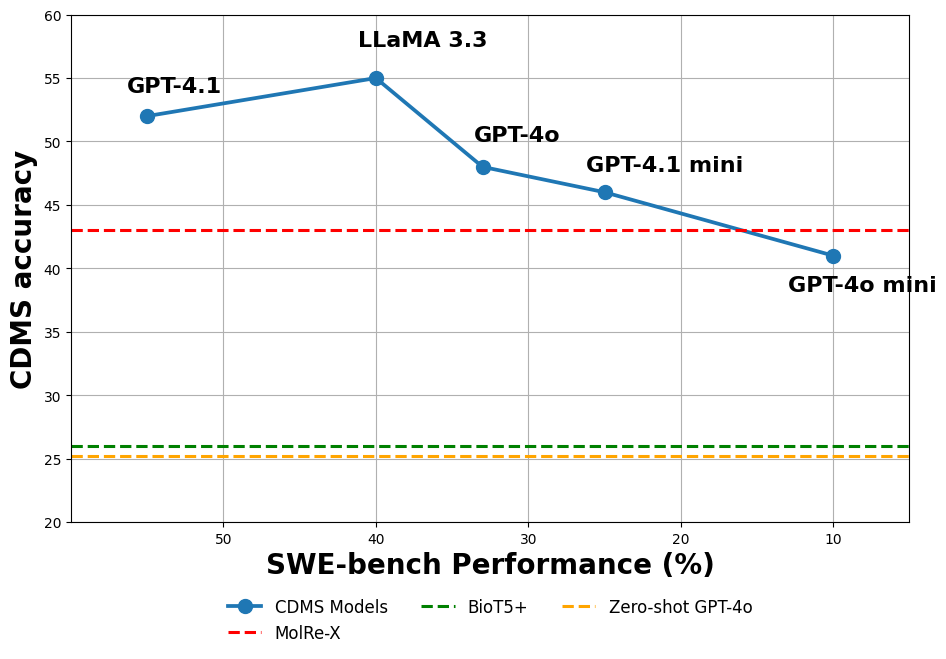
\includegraphics[width=0.4\linewidth]{figures/coder_model_comp (2).png}
        \caption{CDMS performance with weaker coder models.}
        \label{fig:inspector_quality_ablation}
    \end{figure}

\section{Applications of CDMS}
    \subsection{Application to Drug-like Generation}
\label{sec:applications_in_drug}

We compare (i) a one-shot generator that directly maximizes QED and (ii) a two-step, lab-style pipeline: heuristic candidate generation (e.g., limited ring count and no reactive groups) followed by QED filtering, with the QED and SAS computation detailed in Appendix~\ref{app:qed_sas_evaluation}. The former explores a wider chemical space yet often proposes molecules with poor estimated synthetic accessibility; the latter narrows the search but improves SAS.

To quantify the trade-off, we compare state-of-the-art end-to-end molecule generators against a two-stage variant whose first step is either CDMS or one of the molecule-generation baselines considered in this setting. After enforcing expert chemical constraints (Appendix~\ref{app:dataset_samples}), we rank candidates by QED and keep the top 10~\%.  The molecule sampling and post-generation selection procedure used in this experiment is detailed in Appendix~\ref{app:molecule_sampling}. Table~\ref{tab:two_stage_vs_e2e} shows that CDMS delivers both the lowest SAS (best computed synthetic accessibility) and the highest QED (a computational drug-likeness proxy), outperforming BioT5+ and MolReGPT in either setting. We attribute this to the iterative process that builds the molecule gradually. We also note that XlogP (a measure of water solubility) shows that CDMS yields unbiased molecules, as it was not asked to generate soluble molecules, whereas other models produced significantly more soluble compounds — a bias that is not always desirable depending on downstream tasks. Additional optimization results are in Appendix~\ref{app:cdms_opt}.

\begin{table}
    \centering
    \small
    \begin{tabular}{c|l|c|c|c}
        \toprule
        Category & Generative method & SAS ($\downarrow$) & QED ($\uparrow$) & XLogP \\
        \midrule
        \textbf{End-to-End} & BioT5+     & 6.14 & 0.325 & 3.92 \\
                            & MolReGPT   & 2.94 & 0.493 & 4.21 \\
        \midrule
        \textbf{Two-Stage}  & BioT5+     & 3.57 & 0.554 & \textbf{2.71} \\
                            & MolReGPT   & 2.38 & 0.756 & 3.81  \\
                            & CDMS       & \textbf{2.12} & \textbf{0.790} & 3.83 \\
        \bottomrule
    \end{tabular}
    \caption{\small Comparison of end-to-end and two-stage molecule generators across SAS, QED, and XLogP. CDMS was not explicitly prompted to optimize for XLogP, and therefore does not exhibit bias toward this property. Its unbiased performance on XLogP emerges from only satisfying broader user constraints. In contrast, other models were trained on datasets biased toward soluble molecules, which may explain their consistently lower XLogP scores.}
    \label{tab:two_stage_vs_e2e}
\end{table}
    
\section{Generalizing to Other NLP Tasks}
    Our method extends beyond molecular generation to tasks like constrained text generation~\cite{lin-etal-2020-commongen}. To demonstrate this, we designed two new synthetic datasets aimed at addressing LLM limitations in numerical reasoning, structural planning, and constraint adherence.
    \textbf{TextGen} focuses on textual content generation with multi-level constraints, such as ensuring paragraph, sentence limits, and word properties. For example, a task might require creating \textit{"a document with three paragraphs, the first and last being equal in length, and sentences with fewer than 10 words"}. These tasks test the model’s compliance with intricate requirements in text.
    \textbf{StructuredGen} targets structured data generation, requiring models to produce outputs like nested objects or datasets based on detailed specifications. For instance, a task might involve \textit{"generating a list of dictionaries with specific key-value formats and relationships"}. For more examples and details on the generation and structure of these datasets, please see Appendix~\ref{app:nlp_datasets}. Same as in ChemGen, these datasets include a golden inspector code that validates whether a given string adheres to the corresponding textual constraints.

    These datasets challenge LLMs to handle both textual and data-oriented reasoning in a controlled, constraint-driven context.
    
    \subsection{Results}
    We benchmarked CDMS with various underlying generative models against other iterative refinement methods on TextGen and StructuredGen and without iterative refinement. Our results in Table~\ref{tab:textgen_results_summary} show a significant improvement over baseline models in both these tasks as well.  By employing CDMS, we outperform Self-Refine—a text-to-text feedback generation method using LLMs for intermediate reasoning—our approach and Reflexion~\cite{shinn2023reflexion}, which uses reward feedback. Results show a consistent quality improvement trend, with 15\%-44\% gains over the baseline. The quality improvement trend observed in TextGen and StructuredGen was observed across more baselines, please see Appendix~\ref{app:textgen_results}.

    
    \section{Conclusions}
    In this work, we present a novel framework that significantly advances the field of molecular generation by integrating LLMs with an innovative feedback mechanism using Programmatic Feedback Gradients. This iterative feedback loop, powered by an Inspector Model that generates executable validation code, ensures precise compliance with complex, user-defined molecular constraints. Our results demonstrate that CDMS outperforms traditional LLMs and SOTA refinement methods in tasks such as constraint-driven de-novo molecular generation, where adherence to multifaceted structural, functional, and dynamic requirements is critical.
    We contribute our code and dataset to the community for further research.

    For future work, we aim to explore the broader applicability and generalizability of the CDMS framework across various domains. Additionally, we wish to expand CDMS to seamlessly integrate new functionalities, such as instructing the LLM to perform tasks as they are detected. For example, in a molecule reaction-chain detection framework, the LLM could be taught to search for specific chain lengths and provide actionable feedback, all without the need for fine-tuning or additional data. %This can be achieved through in-context learning and few-shot techniques, enabling the model to acquire new abilities in a flexible and efficient manner.

\section{Limitations}
Our method does not directly validate whether the generated code fully captures the intended requirements. Nonetheless, even imperfect code significantly outperforms existing models. Empirically, we found that the generated code enhances LLM performance by providing valuable, targeted feedback. Manual validation revealed that 96\% of inspector code snippets accurately represent the requirements expressed in the original natural language prompts; the measurement protocol, decision-level confusion matrix, and false-positive/false-negative analysis are reported in Appendix~\ref{app:inspector_reliability}. Further discussion on improving code stability and alignment is provided in Section~\ref{sec:enhancing_code_stability}.

One limitation of CDMS is its linear time complexity with respect to the number of refinement attempts (see Section~\ref{sec:cdms}). We believe this can be mitigated through more rigorous prompting strategies, potentially reducing the number of required iterations (see Section~\ref{sec:enhancing_code_stability}). However, as drug discovery is typically not time-sensitive, we consider runtime a secondary concern and prioritize the generation of constraint-compliant molecules. This also marks a shift from traditional iterative refinement, as the feedback in each iteration is not generated by a language model but is instead the result of code execution, enabling more deterministic and verifiable corrections.
A second limitation is that CDMS does not guarantee molecular stability. While the generated molecules may meet specified constraints, they are not necessarily chemically stable. This can be addressed by incorporating domain-specific checks—such as identifying weak bonds or unstable substructures—into the inspector logic. We leave this for future work.
A third limitation is that CDMS cannot validate properties that lack a computable definition. While this constrains the range of enforceable requirements, we conducted an expert review to assess the framework’s practical coverage. Specifically, we asked a domain expert to evaluate which synthesis-relevant properties—drawn from PubChem~\cite{kim2023pubchem}, a public NIH database of chemical structures and properties, and from prior works on molecule synthesis~\cite{fu2021mimosa, pei2024biot5+}—can be encoded in executable code. The expert determined that approximately 50\% of key attributes are directly computable, and an additional 25\% can be estimated using code-accessible deep learning models. The remaining 25\% lack reliable computational methods and were excluded to avoid introducing low-confidence signals. This analysis suggests that CDMS can enforce nearly 75\% of synthesis-relevant properties without requiring lab-based validation, highlighting its practical applicability in computational molecule design. Accordingly, our reported gains reflect satisfaction of computable constraints and computed proxies (e.g., SAS, QED) rather than experimentally measured synthesizability, activity, or drug-likeness. A full breakdown is provided in Appendix~\ref{app:cdms_applicable_features}.

\bibliography{main}
\bibliographystyle{tmlr}

    \appendix


    \section{Prompt and Output Template}
    \label{app:model_prompts}
    We offer a look inside the hood of CDMS. In this work, we leverage foundation models as a code generation model for the inspector component and as a generative model. For reproducibility and transparency, we share the prompts used in our framework. The prompts can be seen per model in Table~\ref{tab:model_prompts}.


    We also share the specific examples used to tune the inspector model.

    \begin{lstlisting}
    from rdkit import Chem
from rdkit.Chem import Descriptors

def check_molecular_weight(mol):
    mw = Descriptors.rdMolDescriptors.CalcExactMolWt(mol)
    if mw < 100:
        needed_increase = 100 - mw
        return f"Molecular weight is {mw:.2f}, which is below 100. Increase it by adding heavier functional groups or atoms to increase by at least {needed_increase:.2f} Da."
    if mw > 200:
        needed_decrease = mw - 200
        return f"Molecular weight is {mw:.2f}, which exceeds 200. Decrease it by removing or replacing functional groups or atoms to decrease by at least {needed_decrease:.2f} Da."
    return None

def check_number_of_atoms(mol):
    num_atoms = mol.GetNumAtoms()
    if num_atoms < 10:
        needed_atoms = 10 - num_atoms
        return f"Number of atoms is {num_atoms}, which is less than 10. Add at least {needed_atoms} more atoms."
    if num_atoms > 50:
        excess_atoms = num_atoms - 50
        return f"Number of atoms is {num_atoms}, which exceeds 50. Remove at least {excess_atoms} atoms."
    return None

def validate_smiles(model_output):
    mol = Chem.MolFromSmiles(model_output)
    if mol is None:
        raise ValueError("Invalid SMILES format.")
    return mol

def check_alcohol_present(mol):
    pattern = Chem.MolFromSmarts('[OX2H]')
    if not mol.HasSubstructMatch(pattern):
        return "Alcohol group (OH) is missing. Consider adding an OH group to the molecule."

def compile_feedback(model_output):
    try:
        mol = validate_smiles(model_output)
        if mol is None:
            return ["Invalid SMILES format. Generate it again to proceed with the validation of other constraints."]
    except Exception as e:
        return [f"Parsing error of the SMILES here is why: {str(e)}. \nGenerate it again to proceed with the validation of other constraints."]

    constraints = [check_number_of_atoms, check_molecular_weight, check_alcohol_present]
    feedback = [constraint(mol) for constraint in constraints]
    # Remove None values
    inspection = [message for message in feedback if message is not None]
    return inspection
    \end{lstlisting}

    
\begin{table*}
    \centering
    \begin{tabular}{|p{2.5cm}|p{13cm}|}
        \hline
        \rowcolor[gray]{0.9} \textbf{Component} & \textbf{Content} \\
        \hline
        \textbf{Generative model} & 
        \textit{You are a skilled chemist tasked with the creation of a new drug.} \\
        & \textit{I will provide you with a list of specific constraints, and your objective is to generate a molecule that meets all of these criteria.} \\
        & \textit{There is always a feasible solution.} \\
        & \textit{You must deliver the result as a SMILES string, ensuring that the molecule you propose is a real, chemically valid compound.} \\
        & \textit{MOST IMPORTANTLY: You must provide only the SMILES string as the output, without any additional characters or information.} \\
        \hline
        \textbf{Inspector} & 
        \textit{You are a code generation model for a chemist researching components. Your task is to generate code from a natural language constraint on molecules that allows me to validate if a certain text complies with the constraints in the prompt.} \\
        & \textit{The code should have one entry point - compile\_feedback that takes in a string and calls all other constraint-checking functions. This function should return a list of the feedback messages from all the constraint-checking functions, and clean the list from None values.} \\
        & \textit{Each constraint-checking function should return a string with textual feedback if the constraint is not met. The textual feedback should describe how the answer violates the constraints this function is checking and how the model can check it. If the text complies, the function should return None.} \\
        & \textit{Make the code return descriptive, actionable textual feedback for each case of the violation and describe how exactly the model should change the output to comply with the constraints.} \\
        & \textit{Include this feedback method always to validate the SMILES of the component.} \\
        & \textit{Make sure you don’t add any example inputs or instance answers in the code.} \\
        & \textit{If the SMILES is invalid, return only the message of invalid SMILES format as feedback. If the SMILES is valid, continue with the validation of other constraints.} \\
        & \textit{Write only the code as a string - do not include any comments or explanations in the code. I will use the code for my purposes.} \\
        \hline
    \end{tabular}
    \caption{Inspector model and generative model prompts.}
    \label{tab:model_prompts}
\end{table*}


    \section{Baseline Training}
    \label{app:baseline_finetuning}

    As mentioned in section~\ref{sec:dataset}, ChemGen has input requirements in natural language, while the target is to generate a molecule that complies with the golden-inspector in each entry. Having this format, ChemGen does not naively support training a model to generate molecules from the textual description. To fine-tune BioT5+, we relied on the raw collected data that ChemGen was created from -- where scraped data about a given molecule has been collected and processed to resemble the input format in ChemGen, where the target was the SMILES of the molecule. Using this aligned data, we trained BioT5+. We trained the proposed BioT5+ for 5 iterations on 60\% of our dataset, with 20\% of it for evaluation, and the rest used for testing.

    

    \section{ChemGen Dataset}
        \label{app:dataset_samples}

Our dataset comprises a set of constraints that a chemist might consider when designing a molecule to satisfy specific properties\cite{guo2024takestangodirectlyoptimizing}. The dataset was constructed using real-world, well-researched molecules through the following steps:

\begin{enumerate}
    \item \textbf{Defining Desired Attributes:} We collaborated with chemists to identify a set of desired attributes that are commonly of interest in molecular design.
    
    \item \textbf{Collecting Molecules:} A total of 779 randomly selected molecules were collected from the PubChem database, covering multiple domains such as salts, industrial building blocks, drug discovery, acids, and more.
    
    \item \textbf{Attribute Annotation:} For each molecule, we retrieved the studied attributes (see Appendix~\ref{app:studied_att}) annotated by human domain experts in the PubChem database. From this, we filtered attributes that matched our predefined set of studied properties.
    
    \item \textbf{Generating Text Descriptions:} Human annotators compiled textual descriptions of the attributes observed in each molecule. For example, a molecule with 2 rings of sizes 2 and 3 and a carboxyl functional group might be described as: \emph{``This molecule has 2 rings, one of size 2 and the other is of size 3, and has a carboxyl functional group.''}
    
    \item \textbf{Code-Based Verification:} Computer scientists annotated these textual constraints to create a \emph{golden-inspector} – a code-based validator. This tool verifies whether a given molecule, represented as a SMILES string, adheres to the textual constraints defined by the dataset.

    \item \textbf{Further Validation:} To further validate the annotated code, we used the source molecule from which the text description—and consequently the code—was generated. We ran the golden-inspector code on this source molecule to ensure there were no errors in dataset creation and to verify that at least one molecule satisfies the \emph{golden-inspector}. Additionally, we conducted a set of experiments to ensure that the code correctly fails for at least one other molecule from the dataset, thereby minimizing the number of false positives.
\end{enumerate}

    Our process ensures the relevancy of the generated constraints and their interest in the domain of de novo molecule generation.

    \subsection{Studied Constraints}
    \label{app:studied_att}
    This section outlines the key constraints in the dataset and their motivations. The source molecule is annotated by $S$
    
    \begin{enumerate}
    \item \textbf{Molecular Weight (MW):} Defines the range of molecular weights to ensure physical and chemical property consistency, critical for solubility, stability, or activity. 
    \[
    \Big[0.8 MW(S) , 1.2MW(S)\Big]
    \]
    
    \item \textbf{Heavy Atoms (HA):} Limits the number of non-hydrogen atoms to control molecular complexity, relevant for drug design and material science. The limit was set as 
    \[
    \Big[max\big(0, HA(S) -2\big) , HA(S)+2\Big]
    \]
    
    \item \textbf{Topological Polar Surface Area (TPSA):} Constrained to predict membrane permeability and solubility, ensuring suitable pharmacokinetic profiles.
    We set the TSPA as
        \[
    \Big[0.8 TPSA(S) , 2TPSA(S)\Big]
    \]

    
    \item \textbf{Covalent Bond Count (CB):} Specifies the total number of covalent bonds between atoms in the molecular graph. This constraint helps control molecular size, structural complexity, and connectivity.
    \[
    \Big[0.8 CB(S) , 1.2 CB(S)\Big]
    \]

    \item \textbf{Rotatable Bonds(RB):} Controls molecular flexibility for balanced rigidity and adaptability, essential for ligand-receptor interactions.
            \[
    \Big[0.8 RB(S) , 1.5 RB(S)\Big]
    \]

    \item \textbf{Rings and Ring Molecules:} Constrains cyclic structures, ensuring structural diversity and alignment with desired properties.
    \[
    \text{rings number} = \Big[max(0,Rn(S)-1) , Rn(S)+2\Big]
    \]
    \[
    \text{ring size} = \Big[ max(0,Rs(S)-2) , Rs(S)+1\Big]
    \]

    
    \item \textbf{Functional Groups:} Enforces inclusion/exclusion of specific functional groups to tailor compounds for various applications. Supported groups include:
\begin{itemize}
    \item \textbf{Alcohol:} -OH (hydroxyl group)
    \item \textbf{Carboxylic Acid:} -COOH (carboxyl group)
    \item \textbf{Ketone:} >C=O (carbonyl group)
    \item \textbf{Aldehyde:} -CHO (formyl group)
    \item \textbf{Amine:} -NH$_2$/-NH- (primary/secondary amine)
    \item \textbf{Amide:} -CONH$_2$ (amide group)
    \item \textbf{Ester:} -COO- (ester group)
    \item \textbf{Ether:} -O- (ether group)
    \item \textbf{Thiol:} -SH (thiol group)
    \item \textbf{Alkene:} C=C (double bond)
    \item \textbf{Alkyne:} C$\equiv$C (triple bond)
    \item \textbf{Phenol:} -C$_6$H$_4$OH (phenolic group)
    \item \textbf{Halide:} -X (halogen atom, where X = F, Cl, Br, or I)
    \item \textbf{Nitrile:} -CN (nitrile group)
    \item \textbf{Sulfonic Acid:} -SO$_3$H (sulfonic acid group)
    \item \textbf{Sulfoxide:} >SO (sulfoxide group)
    \item \textbf{Phosphate:} -PO$_4$ (phosphate group)
    \item \textbf{Nitro:} -NO$_2$ (nitro group)
\end{itemize}
    \end{enumerate}
    
    These constraints ensure dataset relevance for targeted applications while maintaining diversity and utility.
    We contribute our source code and dataset to the community for further research \href{https://anonymous.4open.science/r/CDMS-C08D/}{(here)}. 
    
    \subsection{ChemGen Examples}
    
    Below, we showcase several samples from our dataset. These examples demonstrate how natural language molecule requirements can be translated into corresponding Python code snippets. Each snippet illustrates the implementation of a specific requirement. Please see Table~\ref{tab:requirements} and Table~\ref{tab:additional_requirements} for two examples.

    \begin{table*}[H]
        \centering
        \small
        \begin{tabular}{|p{0.4\textwidth}|p{0.5\textwidth}|}
            \hline
            \textbf{Requirement} & \textbf{Code Snippet} \\
            \hline
            \textbf{1. Covalent bonds count must be less than 9} &
            \begin{lstlisting}[language=Python]
from rdkit import Chem

molecule = Chem.MolFromSmiles(smiles)
result = molecule.GetNumBonds() < 9
            \end{lstlisting} \\
            \hline

            \textbf{2. Topological polar surface area must be greater than 41.206245401121755} &
            \begin{lstlisting}[language=Python]
from rdkit import Chem
from rdkit.Chem import Descriptors

molecule = Chem.MolFromSmiles(smiles)
result = Descriptors.TPSA(molecule) > 41.206245401121755
            \end{lstlisting} \\
            \hline

            \textbf{3. Molecule must not contain Carboxylic Acid} &
            \begin{lstlisting}[language=Python]
from rdkit import Chem

molecule = Chem.MolFromSmiles(smiles)
pattern = Chem.MolFromSmarts('C(=O)O')
result = not molecule.HasSubstructMatch(pattern)
            \end{lstlisting} \\
            \hline

            \textbf{4. Molecule must contain Sulfonic Acid} &
            \begin{lstlisting}[language=Python]
from rdkit import Chem

molecule = Chem.MolFromSmiles(smiles)
pattern = Chem.MolFromSmarts('S(=O)(=O)O')
result = molecule.HasSubstructMatch(pattern)
            \end{lstlisting} \\
            \hline

            \textbf{5. Heavy atom count must be greater than 3 and less than 12} &
            \begin{lstlisting}[language=Python]
from rdkit import Chem

molecule = Chem.MolFromSmiles(smiles)
result = 3 < molecule.GetNumHeavyAtoms() < 12
            \end{lstlisting} \\
            \hline

            \textbf{6. Rotatable bond count must be less than 1} &
            \begin{lstlisting}[language=Python]
from rdkit import Chem
from rdkit.Chem import Descriptors

molecule = Chem.MolFromSmiles(smiles)
result = Descriptors.NumRotatableBonds(molecule) < 1
            \end{lstlisting} \\
            \hline
        \end{tabular}
        \caption{Requirements and corresponding Python code snippets for molecular validation.}
        \label{tab:requirements}
    \end{table*}

    \begin{table*}
        \small
        \centering
        \begin{tabular}{|p{0.4\textwidth}|p{0.5\textwidth}|}
            \hline
            \textbf{Requirement} & \textbf{Code Snippet} \\
            \hline

            \textbf{1. Heavy atom count must be less than 39} &
            \begin{lstlisting}[language=Python]
from rdkit import Chem

molecule = Chem.MolFromSmiles(smiles)
result = molecule.GetNumHeavyAtoms() < 39
            \end{lstlisting} \\
            \hline

            \textbf{2. Molecular weight must be less than 383.4636744835153} &
            \begin{lstlisting}[language=Python]
from rdkit import Chem
from rdkit.Chem import Descriptors

molecule = Chem.MolFromSmiles(smiles)
weight = Descriptors.rdMolDescriptors.CalcExactMolWt(molecule)
result = weight < 383.4636744835153
            \end{lstlisting} \\
            \hline

            \textbf{3. Topological polar surface area must be less than 73.27746879710806} &
            \begin{lstlisting}[language=Python]
from rdkit import Chem
from rdkit.Chem import Descriptors

molecule = Chem.MolFromSmiles(smiles)
result = Descriptors.TPSA(molecule) < 73.27746879710806
            \end{lstlisting} \\
            \hline

            \textbf{4. Molecule must have 1 ring of size 6} &
            \begin{lstlisting}[language=Python]
from rdkit import Chem
from collections import Counter

molecule = Chem.MolFromSmiles(smiles)
rings = molecule.GetRingInfo().AtomRings()
ring_sizes = [len(ring) for ring in rings]
ring_counter = Counter(ring_sizes)
result = ring_counter.get(6, 0) == 1
            \end{lstlisting} \\
            \hline

            \textbf{5. Molecule must not contain Phosphate} &
            \begin{lstlisting}[language=Python]
from rdkit import Chem

molecule = Chem.MolFromSmiles(smiles)
pattern = Chem.MolFromSmarts('P(=O)(O)(O)[#6]')
result = not molecule.HasSubstructMatch(pattern)
            \end{lstlisting} \\
            \hline

        \end{tabular}
        \caption{Additional requirements and corresponding Python code snippets for molecular validation.}
        \label{tab:additional_requirements}
    \end{table*}


    \section{Inspector Reliability: Agreement with Golden Validators}
    \label{app:inspector_reliability}

    Because the generated inspector $M_I$ drives the refinement loop, its reliability is central to CDMS. We therefore quantify how closely a \emph{generated} inspector reproduces the decisions of the hand-verified \emph{golden} validator constructed during dataset annotation (Appendix~\ref{app:dataset_samples}).

    \paragraph{Measurement protocol.}
    We evaluate inspector reliability using \emph{behavioral equivalence} rather than manual code inspection, thereby assessing each inspector by its decisions. For each ChemGen item, we generate an inspector code using $M_I$ and evaluate it on a fixed probe set of $1{,}000$ molecules. The probe set includes the source molecule from which the sample was constructed, which satisfies the golden validator by construction, as well as $999$ additional molecules selected to induce both accepting and rejecting outcomes. We execute the generated inspector and the corresponding golden validator on every probe molecule and record their binary accept/reject decisions. We consider a generated inspector accurate for an item if and only if its decisions agree with those of the golden validator on all $1{,}000$ probe molecules; that is, the two validators are behaviorally equivalent over the probe set. 
    
    The reported accuracy of $96\%$ is the proportion of the 779 generated inspectors that satisfy this criterion

    \paragraph{False positives and false negatives.}
    To characterize the residual \textcolor{red}{[PLACEHOLDER: $\approx 4$]}\% of non-equivalent inspectors, we analyze disagreements at the level of individual (inspector, molecule) decisions, taking the golden validator as ground truth. A \emph{false positive} (FP) is a molecule accepted by the generated inspector but rejected by the golden validator, whereas a \emph{false negative} (FN) is a molecule rejected by the generated inspector but accepted by the golden validator. Table~\ref{tab:inspector_confusion} reports the aggregated confusion matrix over all probe decisions together with the induced false-positive rate $\mathrm{FPR}=\mathrm{FP}/(\mathrm{FP}+\mathrm{TN})$ and false-negative rate $\mathrm{FNR}=\mathrm{FN}/(\mathrm{FN}+\mathrm{TP})$.

    \begin{table}[h]
        \centering
        \small
        \begin{tabular}{l|cc}
            \toprule
             & \multicolumn{2}{c}{Golden validator} \\
            Generated inspector & Accept & Reject \\
            \midrule
            Accept & TP $=$ \textcolor{red}{[\,..\,]} & FP $=$ \textcolor{red}{[\,..\,]} \\
            Reject & FN $=$ \textcolor{red}{[\,..\,]} & TN $=$ \textcolor{red}{[\,..\,]} \\
            \bottomrule
        \end{tabular}
        \caption{Decision-level agreement between the generated inspector and the golden validator over the probe molecules, with the golden validator taken as ground truth. \textcolor{red}{[PLACEHOLDER: insert TP/FP/FN/TN counts; resulting $\mathrm{FPR}=$\,..\,\%, $\mathrm{FNR}=$\,..\,\%.]}}
        \label{tab:inspector_confusion}
    \end{table}

    \paragraph{Error categories.}
    We additionally classify each non-equivalent inspector by the source of its disagreement with the golden validator: \textbf{(i)} \emph{incomplete coverage}, where a constraint named in the requirement is not checked by the generated code; \textbf{(ii)} \emph{over-strict checks}, where the generated code enforces a tighter condition than intended (the dominant source of false negatives); \textbf{(iii)} \emph{over-permissive checks}, where the generated code omits or relaxes a condition (the dominant source of false positives); and \textbf{(iv)} \emph{implementation errors}, e.g., an incorrect SMARTS pattern or property threshold. \textcolor{red}{[PLACEHOLDER: report the count/fraction of non-equivalent inspectors in each category.]}


    \section{CDMS for Drug Like End-to-End Molecular Generation}
    \label{app:cdms_opt}

    \subsection{CDMS to optimize drug-like aspects}
    
    We conducted an experiment to demonstrate that CDMS, with $M_G = $GPT-4o, can optimize specific attributes of generated molecules when prompted. To do this $M_I$ was supplied with external prediction tools to incorporate as inspectors. We incorporated into the inspector model’s prompt how to use the tool, while the evaluation was delegated to the specialized model.
    
    In this experiment we asked the model in the form of text to optimize attributes in the molecule such as synthesizability (SAS), drug likeness (QED), and solubility in water (LogP). The target was to optimize beyond the average achieved without filtering by CDMS. The full results are shown in Table~\ref{tab:optimized-CDMS-molecule-sorting}. BioT5+ and MolReGPT were not designed to optimize particular molecular aspects, and as a result, we observed no notable improvements when textual optimization was attempted via text requirement which led to their exclusion from this table. CDMS, however, successfully optimized each aspect when using the predictor as a code inspector within the optimization process. Regarding constraint adherence accuracy, we did not observe any degradation. We note that the additional constraints led to an increase in the allowed number of optimization attempts, which was set to 10 to compensate for the more complex constraints.
    
    \begin{table}[H]
        \centering
        \small % Reduce font size to ensure it fits in a single column
        \begin{tabular}{l|c|c|c|c|c|c}
            \toprule
            \multirow{3}{*}{\parbox{1.5cm}{\centering \textbf{Generative Model}}} & \multicolumn{2}{c|}{\textbf{SAS($\downarrow$)}} & \multicolumn{2}{c|}{\textbf{QED($\uparrow$)}} & \multicolumn{2}{c}{\textbf{LogP($\downarrow$)}} \\
            \cmidrule(lr){2-3} \cmidrule(lr){4-5} \cmidrule(lr){6-7}
            & \textbf{Avg} & \textbf{Top 10\%} & \textbf{Avg} & \textbf{Top 10\%} & \textbf{Avg} & \textbf{Top 10\%} \\
            \midrule
            CDMS (SAS opt) & 3.09  & \textbf{1.39} & 0.44 & 0.71 & 1.39 & -0.39 \\ 
            CDMS (QED opt) & \textbf{2.91} & 1.83 & \textbf{0.51} & \textbf{0.75} & 4.98 & 0.92 \\ 
            CDMS (LogP opt) & 4.10 & 1.79 & 0.419 & 0.57 & \textbf{1.09} & \textbf{-0.96} \\ 
            \bottomrule
        \end{tabular}
        \caption{\small Performance of CDMS under different optimization criteria (SAS, QED, LogP).}
        \label{tab:optimized-CDMS-molecule-sorting}
    \end{table}
    
    \subsection{Generative model SAS quality}
    We evaluated the SAS scores of the molecules generated by each generative model in Section~\ref{sec:applications_in_drug}. Notably, CDMS demonstrated the ability to consistently generate molecules within the low-SAS region. We notice that BioT5+ mainly produces high-SAS molecules, reflecting the strengths of CDMS.

    

    
    
        \section{NLP domain datasets}
    \label{app:nlp_datasets}

    \subsection{TextGen}
    The TextGen dataset is designed to evaluate the performance of large language models (LLMs) in numerical reasoning and compliance with textual constraints. For instance, a sample task could be: \textit{"Create a document with \textbf{three} sections. The \textbf{first} and \textbf{last} sections should be of \textbf{equal length}, while the \textbf{second} section must be at least \textbf{twice as long}. Ensure that each \textbf{sentence} contains \textbf{fewer than 10 words}, and each word has \textbf{fewer than 7 letters}."}
    Such prompts can be employed for generating simplified reading material for children, the use cases are endless.
    Similar to the ChemGen dataset, TextGen incorporates both hierarchical textual constraints and golden inspectors to verify compliance with these constraints. The constraints are organized across multiple levels:
    \begin{itemize}
        \item \textbf{Document level:} Limits overall document length and the number of paragraphs. 
        \item \textbf{Paragraph level:} paragraph length and the number of sentences restrictions. 
        \item \textbf{Sentence level:} Constraints on the number of words per sentence.
        \item \textbf{Word and sub-word level:} Requirements on word length, part-of-speech, and syllable counts.
    \end{itemize}
    
    To further increase task complexity and assess reasoning over hierarchical constraints, each entity that imposes requirements on its sub-entities employs an aggregation method. The supported methods are as follows:
    \begin{itemize}
        \item \textbf{None:} None of the sub-requirements must be met.
        \item \textbf{All:} All sub-requirements must be met.
        \item \textbf{At-least-X:} At least $X$ sub-requirements must be satisfied.These methods challenge the model's ability to reason about and comply with intricate constraints.
    \end{itemize}
    
    The iterative feedback mechanism, initially proposed for CDMS, has also proven to be effective for TextGen. A straightforward prompt modification (see Appendix~\ref{app:ICICLE_textgen_prompts} for the specific prompts) enables the model to surpass prior SOTA results in content generation while maintaining compliance with the specified constraints.
        
    \subsection{StructuredGen}
    While the previous dataset (TextGen) focuses on generating text with hierarchical constraints, StructuredGen targets the generation of structured content such as objects, data classes, or entire datasets. For example, a task might require the LLM to generate a structured data type with the following specifications: " \textit{A \textbf{list} containing a \textbf{dictionary} with: (1) \textbf{three} entries where the \textbf{key is a float} and the value is a \textbf{list of three strings}, and (2) \textbf{four entries} where the \textbf{key is a string} and the \textbf{value is a dictionary} with specific entries.}"
        
    To evaluate LLMs' ability to manage data complexities, we define two primary classes of data types:
    \begin{enumerate}
        \item \emph{Terminal types:} One of \texttt{[int, float, str]}.
        \item \emph{Complex types:} One of \texttt{[list, dict]}.
    \end{enumerate}
    
    As in TextGen, constraints must be satisfied across the data hierarchy, including aggregation requirements on sub-entities. This ensures the generated output adheres to the specified conditions and integrates multiple constraints seamlessly.
    

    
    
    \section{TextGen and StructuredData Results}
    \label{app:textgen_results}
    We conducted a human evaluation on a sample of the generated content, asking participants to assess the quality of each passage without being informed of the number of iterations involved in the optimization process. The results indicate that the iterative refinement process does not impact the perceived quality of the generated content. Figure~\ref{fig:iterative_quality_in_textgn} presents the normalized scores assigned by the human annotators to the evaluated models.
    The human evaluation to assess the quality of the generated text observed no significant deterioration in quality after five iterations—the maximum number of allowed attempts for this task. The human evaluators were graduate and undergraduate students of engineering who volunteered to annotate this task for scientific purposes. The full evaluation prompt was as follows: "Rate the following content based on its logical flow, vocabulary usage, and overall quality. Provide a score between 1 and 5, with 5 being the highest.".

    The overall quality measured by the proportion of outputs that would be accepted by the golden inspector is shown in Figure~\ref{fig:iterative_quality_in_textgn}.

    \begin{table*}
    \centering
    \small
    \begin{tabular}{p{1.4cm} l|p{1.4cm}|p{1.4cm}|p{1.4cm}|p{1.25cm}|>{\columncolor{gray!20}}p{1.25cm}|>{\columncolor{gray!20}}p{1.25cm}}
        \toprule
        Dataset      & Method   & GPT4o (1.7T)    & LLama-3.1 (405B) & Phi3-medium (14B) & Mistral (7B)   & GPT4o with CoT & GPT4o with K-shot \\
        \midrule
        {Structured-Gen} & Base                               & 31.12          & 34.52            & 15.55             & 12.44          & 31.76          & 33.48 \\
        {}           & Self-Refine\cite{madaan2024self}   & 32.14          & 35.07            & 20.53             & 13.14          & 33.13          & 33.47 \\
        {}           & Reflexion\cite{shinn2023reflexion} & 33.51          & 34.73            & 18.13             & 14.41          & 34.47          & 36.36 \\
        {}           & CDMS (Ours)                        & \textbf{35.92} & \textbf{49.44}   & \textbf{24.02}    & \textbf{18.91} & \textbf{37.02} & \textbf{41.61} \\

        \midrule
        {TextGen}    & Base                               & 53.91          & 49.23            & 28.05             & 30.61          & 56.13          & 55.75 \\
        {}           & Self-Refine\cite{madaan2024self}   & 54.61          & 50.21            & 40.12             & 31.62          & 57.26          & 58.62 \\
        {}           & Reflexion\cite{shinn2023reflexion} & 55.23          & 51.24            & 37.34             & 29.55          & 57.14          & 59.52 \\
        {}           & CDMS (Ours)                        & \textbf{62.65} & \textbf{57.35}   & \textbf{55.23}    & \textbf{44.10} & \textbf{64.05} & \textbf{70.52} \\
        \bottomrule
    \end{tabular}
    \caption{\small Averaged Performance of Models Across Datasets}
    \label{tab:textgen_results_summary}
\end{table*}

    

    \section{Natural Language Constrained Generation Dataset}
    \label{sec:textgen_dataset}
    We propose two new datasets to highlight the shortcomings of current LLMs, particularly in numerical reasoning, structural planning, and adherence to complex requirements. These datasets are:

    \begin{itemize}
        \item \textbf{TextGen Dataset:} Designed for free-text generation under hierarchical constraints.
        \item \textbf{Structured Content Dataset:} Focuses on generating structured data, such as lists and dictionaries, adhering to specific requirements.
    \end{itemize}

    The tasks are split into easy and hard versions to accommodate varying complexity levels. Easy tasks mirror typical day-to-day constraints (e.g., \enquote{Create a text about flowers with at least 100 words and fewer than 120 words}). Hard tasks stress-test models with intricate requirements (e.g., \enquote{Write a Haiku where each verse starts and ends with the same two letters, with 5 verses mentioning 'tree' exactly once in each}).

    \subsection{Dataset Versions and Goals}
    \label{subsec:dataset_versions}
    Our datasets serve to:
    \begin{enumerate}
        \item Exemplify challenges LLMs face when handling complex instructions.
        \item Showcase how our method overcomes these challenges by generating code to meet stringent criteria.
    \end{enumerate}

    \subsection{TextGen Dataset}
    \label{subsec:textgen_dataset}
    The TextGen dataset evaluates the structural comprehension and numerical reasoning capabilities of LLMs in free-text generation tasks. Examples include generating paragraphs, sentences, and words under specific constraints. For instance:

    \begin{figure}[h]
        \centering
        \begin{tcolorbox}[colback=gray!20, colframe=black, width=\linewidth, sharp corners]
            Generate a text that satisfies the following constraints:
            \begin{enumerate}
                \item A paragraph that both starts and ends with the same word.
                \item A paragraph that contains at least three sentences.
            \end{enumerate}
        \end{tcolorbox}
        \caption{Example Text Generation Constraints}
        \label{fig:text_const_app}
    \end{figure}

    \subsection{Structured Content Dataset}
    \label{subsec:structured_dataset}
    The Structured Content Dataset focuses on generating structured data types, such as lists and dictionaries, with specific constraints. For example:

    \begin{figure}[h]
        \centering
        \begin{tcolorbox}[colback=gray!20, colframe=black, width=\linewidth, sharp corners]
            Generate a structured data type that includes:
            \begin{itemize}
                \item A list containing a dictionary with the following entries:
                \begin{itemize}
                    \item Three entries where the key is a float and the value is a list containing three strings.
                    \item Four entries where the key is a string and the value is a dictionary with specific entries.
                \end{itemize}
            \end{itemize}
        \end{tcolorbox}
        \caption{Example Structured Data Generation Description}
        \label{fig:data_structure}
    \end{figure}

    The dataset includes tasks to test LLMs' ability to manage terminal data types (e.g., \texttt{int}, \texttt{float}, \texttt{str}) and complex data types (e.g., \texttt{list}, \texttt{dict}).


    % \section{Memory JSON format}
    % \label{sec:memeory_format}
    % Memory within our system is managed as a JSON object, structured as an alternating dictionary. This dictionary distinctly catalogs the interactions between two main components: the generative model, labeled as "assistant," and the inspector model, labeled as "user." This format efficiently organizes and maintains the dialogue between these components, facilitating smooth and effective communication. Figure~\ref{fig:memeory_format}.
    
    \section{TextGen Prompt}
    \label{app:ICICLE_textgen_prompts}
    We aimed to evaluate the applicability of CDMS in constrained natural language generation. To this end, we used the same architecture while modifying only the prompting, as detailed in Table~\ref{tab:icicle_prompts}. Additionally, we included a few-shot example to both the generative model and the inspector model from the dataset to better tune the model.
    
\begin{table*}[t]
    \centering
    \begin{tabular}{|p{2.5cm}|p{13cm}|}
        \hline
        \rowcolor[gray]{0.9} \textbf{Component} & \textbf{Content} \\
        \hline
        \textbf{Generative model} & 
        \textit{You are a skilled \textbf{[ Text generation/Json Data generation ]} tasked with the creation of a new drug \textbf{[Data]}.} \\
        & \textit{I will provide you with a list of specific constraints, and your objective is to generate a \textbf{[Data]} that meets all of these criteria.} \\
        & \textit{There is always a feasible solution.} \\
        & \textit{\sout{You must deliver the result as a SMILES string, ensuring that the molecule you propose is a real, chemically valid compound.}} \\
        & \textit{MOST IMPORTANTLY: You must provide only the \sout{SMILES} string as the output, without any additional characters or information.} \\
        \hline
        \textbf{Inspector} & 
        \textit{You are a code generation model for a \textbf{[Natural Text generation / Json Generation]}. Your task is to generate code from a natural language constraint on molecules that allows me to validate if a certain text complies with the constraints in the prompt.} \\
        & \textit{The code should have one entry point - compile\_feedback that takes in a string and calls all other constraint-checking functions. This function should return a list of the feedback messages from all the constraint-checking functions, and clean the list from None values.} \\
        & \textit{Each constraint-checking function should return a string with textual feedback if the constraint is not met. The textual feedback should describe how the answer violates the constraints this function is checking, and how the model can check it. If the text complies, the function should return None.} \\
        & \textit{Make the code return descriptive, actionable textual feedback for each case of the violation and describe how exactly the model should change the output to comply with the constraints.} \\
        & \textit{Include this feedback method always to validate the SMILES of the component.} \\
        & \textit{Make sure you don’t add any example inputs or instance answers in the code.} \\
        & \textit{If the SMILES is invalid, return only the message of invalid SMILES format as feedback. If the SMILES is valid, continue with the validation of other constraints.} \\
        & \textit{Write only the code as a string - do not include any comments or explanations in the code. I will use the code for my purposes.} \\
        \hline
    \end{tabular}
    \caption{Inspector model and generative model prompts in TextGen and structured data generation tasks.}
    \label{tab:icicle_prompts}
\end{table*}

    
    \begin{figure}
        \centering
        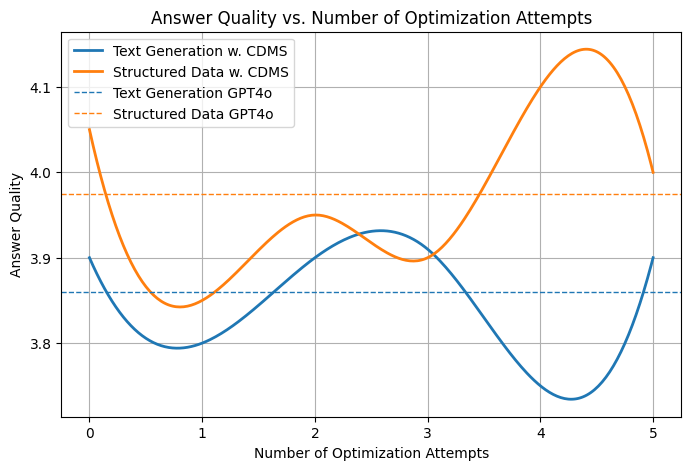
\includegraphics[width=0.5\linewidth]{figures/texge_quality.png}
        \caption{Normalized content quality of generated answers after a number of optimization attempts}
        \label{fig:iterative_quality_in_textgn}
    \end{figure}
    
    \lstset{
        basicstyle={\footnotesize\ttfamily},
        frame=tb,
        backgroundcolor=\color{gray!10}    % Background color, light gray
    }
    \begin{lstlisting}
        [ {"role": "user", "content": <'content'>},
        {"role": "assistant", "content": <'content'>} ]
    \end{lstlisting}
    \label{fig:memeory_format}
        
    \section{Model hyperparameter}
    The hyperparameter tuning process for our model involved extensive experimentation to ensure optimal performance while minimizing reliance on collected data. Below, we summarize the key findings and decisions made during this process:

    \paragraph{Number of Iterations for CDMS}
    Initially, the maximum allowed number of iterations for CDMS was set to 20. However, using a validation set (separate from the test set), we determined that the optimal number of iterations is 7.

    \paragraph{Few-Shot Examples}
    We experimented with the number of few-shot examples provided to the model. The goal was to identify the minimal number of examples required to achieve the best results while reducing dependency on collected data. For the inspector code generation model, where the model generates code from the textual requirements that is largely self-explanatory, we found that extensive examples were unnecessary. Instead, we provided a schema illustrating the expected code structure. This schema included functions for validating each constraint, with a return value of type string.

    The model, guided by this schema, automated the remainder of the code generation process with high accuracy (96\%). This result highlights the efficacy of our approach in leveraging minimal input to achieve reliable outcomes.


    \section{Implementation Details}
    The CDMS code was implemented using Python 3.10. Chemistry knowledge for data collection and inspection was powered by RDKit\cite{rdkit} version 2022.9.4, a Python toolkit enabling real-time querying of chemical components. However, we observed that the generated inspector code occasionally relied on PubChempy\cite{kim2023pubchem}, and deepchem\cite{deepchem}, but we cannot be sure which package it used in every scenario.

    For model deployments, we utilized Azure OpenAI for GPT-4o and Qwen, Anthropic's API for Claude, and NVIDIA NIM for LLaMA.

    Inference for the whole dataset costs less than 40\$ using the AzureOpenAI and NVIDIA NIM.

    \subsection{QED and SAS Evaluation}
    \label{app:qed_sas_evaluation}
    
    We compute QED and synthetic accessibility scores using RDKit version 2024.09.1. Each generated SMILES string is parsed with \texttt{Chem.MolFromSmiles}, and invalid molecules are excluded from these calculations.
    
    QED is computed with \texttt{rdkit.Chem.QED.qed} and ranges from 0 to 1, where higher values indicate greater drug-likeness.
    
    Synthetic accessibility (SAS) is computed with RDKit's implementation of the Ertl--Schuffenhauer score, \texttt{rdkit.Contrib.SA\_Score.sascorer.calculateScore}. We denote this metric as SAS, which ranges from 1 to 10, where lower values indicate greater estimated synthetic accessibility.
    
    Both metrics are deterministic functions of the molecular graph and are used as computational proxies rather than evidence of experimental drug-likeness or the existence of a feasible synthesis route.
    
\section{Molecule Sampling} \label{app:molecule_sampling}

In this experiment, we utilized GPT-4o in a zero-shot setting to generate candidate molecules and also as the backbone for inspector-code generation. For each given set of constraints in ChemGen, we first sampled 500 candidate molecules using GPT-4o as the generative model. The generative model was not explicitly instructed to optimize for any specific molecular attribute, such as SAS, QED, or LogP, during this sampling stage. After the candidate molecules were generated, we used GPT-4o to generate the corresponding inspector code, denoted as $M_I$, for the same set of constraints. The generated inspector was then used as a first-stage filter over the 500 sampled molecules.

\subsection{Accuracy}

The first-stage filtering pass rate was 46.00\%. That is, 46.00\% of the 500 zero-shot sampled molecules passed the validation of the generated inspector $M_I$. This number reflects only the acceptance rate of the first filtering phase and should not be interpreted as the end-to-end accuracy of CDMS or as accuracy with respect to the golden-standard inspector code.

\subsection{Molecule Selection}

After applying the first-stage filter, we selected molecules from the sampled candidates based on their scores for each metric---SAS, QED, and LogP---using a predictive scoring model (see~\ref{app:qed_sas_evaluation}. Specifically, we selected the top 10\% of the original sampled pool, corresponding to 50 molecules, for each metric. The results indicate that these molecular properties could be effectively optimized through post-generation selection, even though the generative model was not explicitly prompted to optimize them during the initial sampling stage. Furthermore, 44\% of the selected molecules passed the generated-inspector filter, suggesting that property-based selection did not substantially reduce the first-stage filtering pass rate.

\section{Molecule synthesis applicable features}
\label{app:cdms_applicable_features}
To assess the practical applicability of the CDMS framework, we examined its coverage over key aspects of small molecule synthesis and drug discovery. Since CDMS employs code-enabled feedback mechanisms and integrates deep learning models, it is essential to evaluate how well it supports real-world chemical workflows.\\
To this end, we partnered with expert chemists to identify a representative set of features most commonly used in medicinal chemistry. These features span structural, biological, and pharmacological properties. Table~\ref{tab:chem_synthesis_descriptors} summarizes the structural and physicochemical properties, while Table~\ref{tab:bioactivity_attributes} presents attributes related to molecular bioactivity. These aspects are further annotated to indicate whether they are computable via code (e.g., using RDKit), predictable using learned models, or require experimental validation.

\begin{table*}[ht]
\centering
\begin{tabular}{|l|c|}
\hline
\textbf{Attribute} & \textbf{How It Can Be Verified} \\
\hline
\multicolumn{2}{|c|}{\textbf{Structural and Physicochemical Properties}} \\
\hline
Molecular Formula & Code (100\% accurate) \\
Molecular Weight & Code (100\% accurate) \\
Exact Mass & Code (100\% accurate) \\
Monoisotopic Mass & Code (100\% accurate) \\
Formal Charge & Code (100\% accurate) \\
Topological Polar Surface Area (TPSA) & Code (100\% accurate) \\
Rotatable Bond Count & Code (100\% accurate) \\
Hydrogen Bond Donor/Acceptor Count & Code (100\% accurate) \\
Complexity Score & Code (100\% accurate) \\
Vapor Density (est.) & Code (100\% accurate) \\
Oxidation Behavior (functional group level) & Code (100\% accurate) \\
Number of Heavy Atoms & Code (100\% accurate) \\
Number of Aromatic Rings & Code (100\% accurate) \\
Number of Aliphatic Rings & Code (100\% accurate) \\
Number of Saturated Rings & Code (100\% accurate) \\
Number of Ring Systems & Code (100\% accurate) \\
Number of Bridgehead Atoms & Code (100\% accurate) \\
Number of Spiro Atoms & Code (100\% accurate) \\
Number of Heteroatoms & Code (100\% accurate) \\
Number of Nitrogens and Oxygens & Code (100\% accurate) \\
Number of Valence Electrons & Code (100\% accurate) \\
Number of Radical Electrons & Code (100\% accurate) \\
Fraction of Csp3 Carbons & Code (100\% accurate) \\
Ring Count & Code (100\% accurate) \\
\hline
\multicolumn{2}{|c|}{\textbf{Predicted or Approximate Properties}} \\
\hline
XLogP3 (predicted LogP) & Code (high probability) \\
1H NMR Spectrum (predicted) & Code (high probability) \\
Physical State (approx.) & Code (high probability) \\
Primary Hazard Estimation (QSAR-based) & Code (high probability) \\
Volatility with Steam & Code (high probability) \\
Boiling Point (predicted) & Code (medium–low accuracy) \\
Melting Point (predicted) & Code (medium–low accuracy) \\
Solubility in Water (predicted) & Code (medium–low accuracy) \\
pKa (predicted) & Code (medium–low accuracy) \\
Flash Point (predicted) & Code (medium–low accuracy) \\
Vapor Pressure (predicted) & Code (medium–low accuracy) \\
\hline
\multicolumn{2}{|c|}{\textbf{Properties Requiring Experimental Validation}} \\
\hline
LogP (experimental) & Lab required \\
Boiling Point (true) & Lab required \\
Melting Point (true) & Lab required \\
Solubility (true) & Lab required \\
pKa (accurate value) & Lab required \\
Flash Point (certified) & Lab required \\
Vapor Pressure (precise) & Lab required \\
Reduction Behavior (e.g., silver nitrate test) & Lab required \\
Shelf Stability & Lab required \\
1H NMR Spectrum (measured) & Lab required \\
MS Spectrum & Lab required \\
IR Spectrum & Lab required \\
\hline
\end{tabular}
\caption{Verification modes of synthesis-relevant molecular attributes}
\label{tab:chem_synthesis_descriptors}
\end{table*}


\begin{table*}[ht]
\centering
\begin{tabular}{|l|c|}
\hline
\textbf{Biological/Pharmacological Aspect} & \textbf{How It Can Be Verified} \\
\hline
Blood–Brain Barrier Permeability & Code (high probability) \\
General Toxicity (e.g., Tox21) & Code (high probability) \\
High-Throughput Toxicity (e.g., ToxCast) & Code (high probability) \\
Virtual Screening Effectiveness (e.g., MUV) & Code (high probability) \\
HIV Inhibition Activity & Code (high probability) \\
Beta-Secretase Inhibition (BACE) & Code (high probability) \\
Side Effect Likelihood (e.g., SIDER) & Code (medium–low accuracy) \\
Clinical Toxicity Risk (e.g., ClinTox) & Code (medium–low accuracy) \\
Aggregate Bioactivity Score & Code (high probability) \\
\hline
\end{tabular}
\caption{Verification modes of biological and pharmacological molecular properties}
\label{tab:bioactivity_attributes}
\end{table*}

\section{Application of CDMS in Drug Discovery}
\label{app:applications}

\begin{figure*}
    \centering
    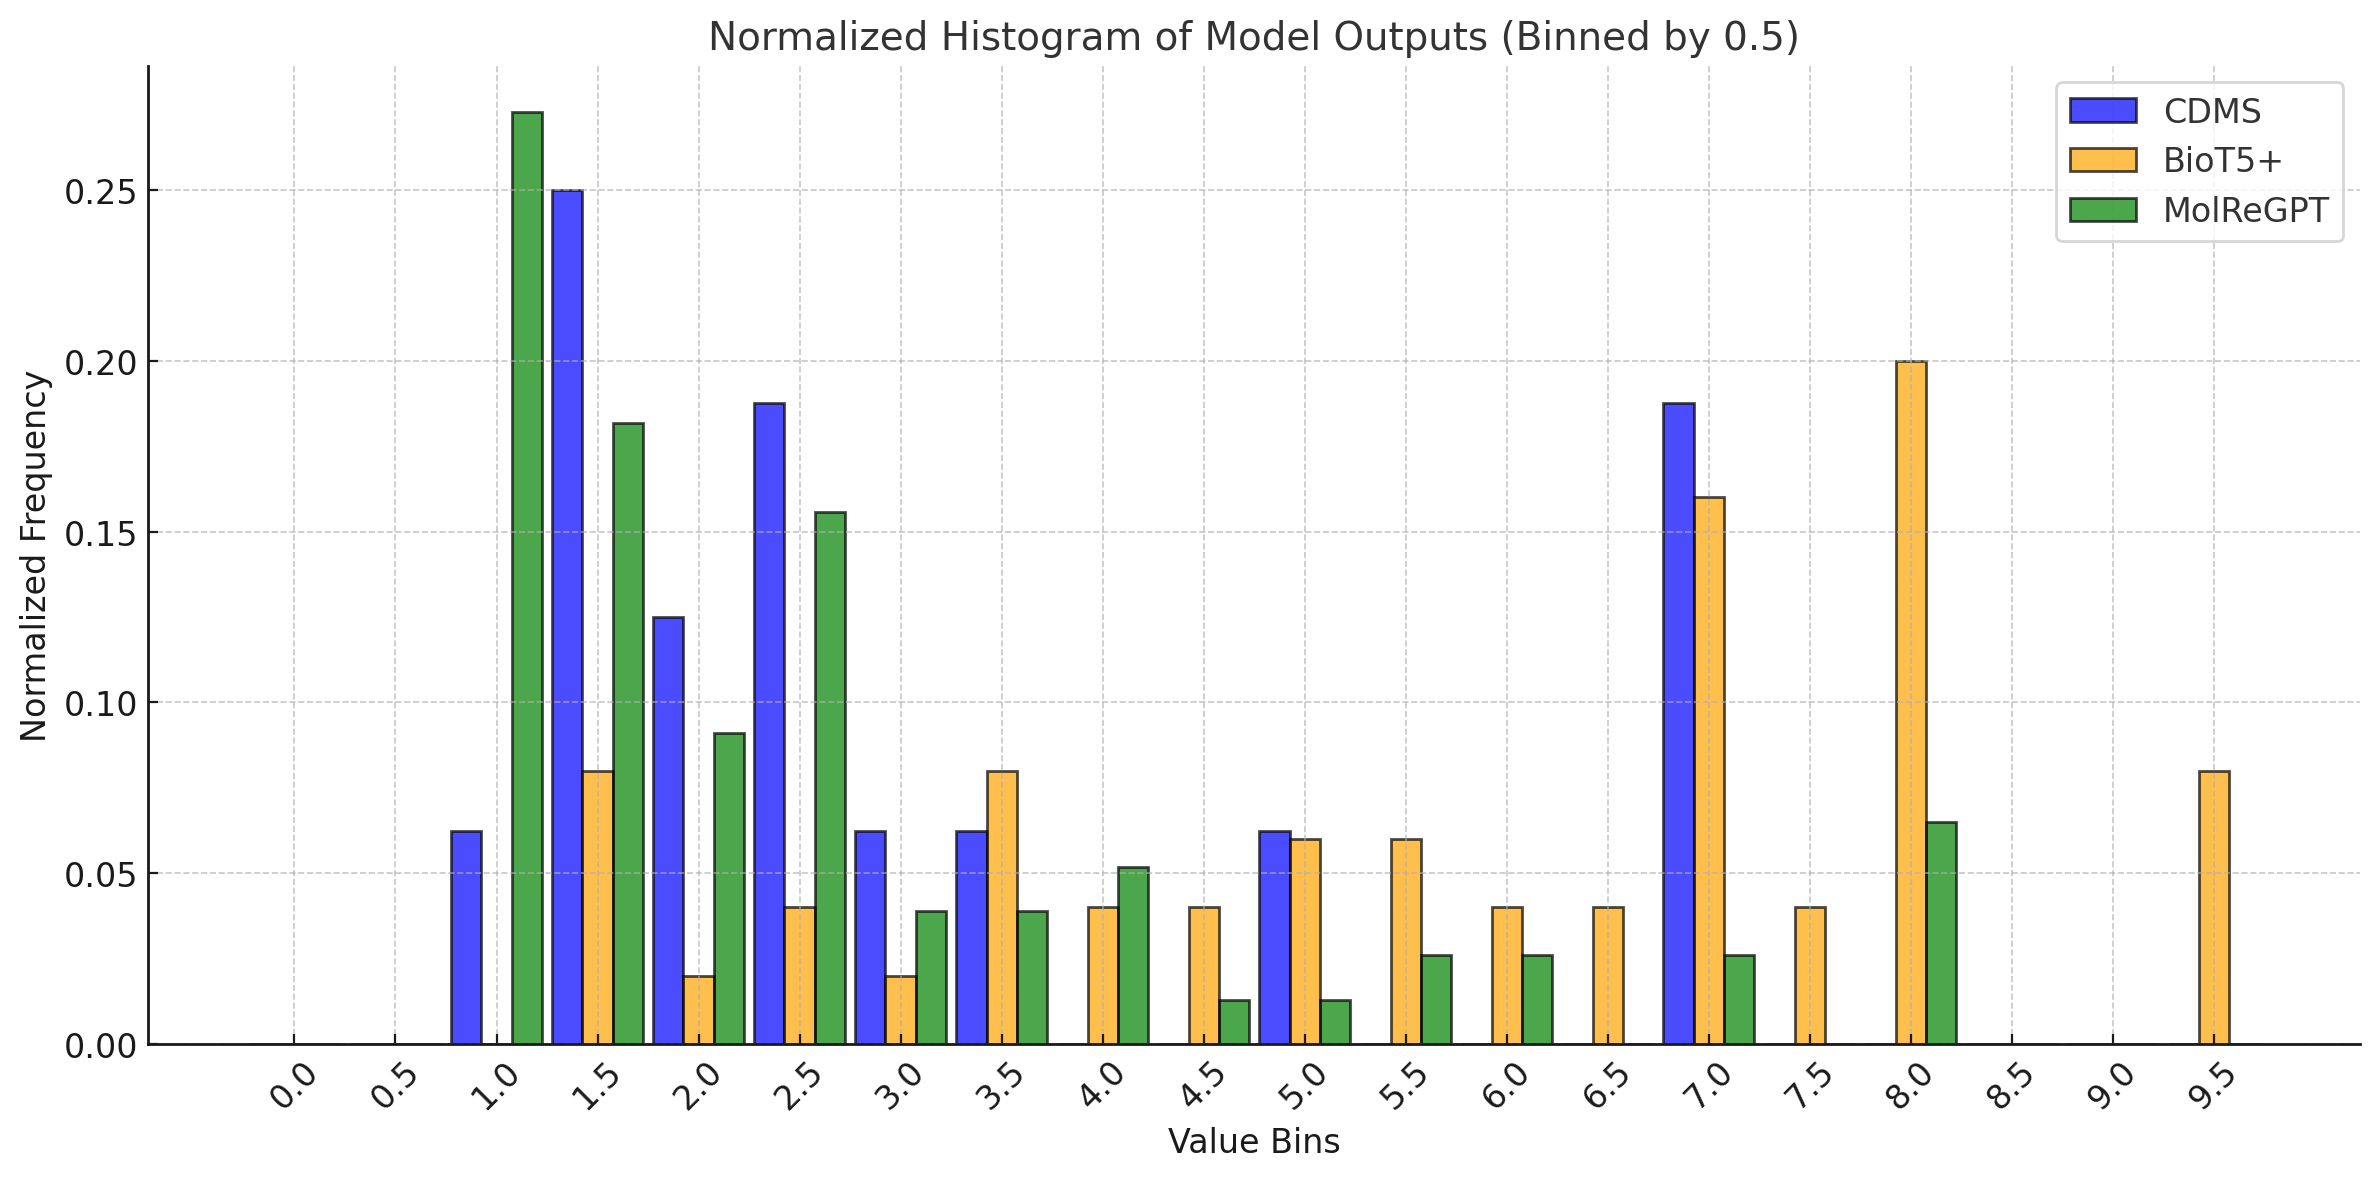
\includegraphics[width=1\linewidth]{figures/output.png}
    \caption{SAS normalized distribution of generated molecules using different generative models}
    \label{fig:sas_score_hist}
\end{figure*}

We evaluated the applicability of CDMS in the domain of drug discovery by instructing the model to optimize specific aspects of the generated molecules, namely SAS, QED, and LogP, while adhering to the constraints provided in each sample from the ChemGen dataset. The inspector model $M_I$ was equipped with a predictive method capable of estimating the score for each of these aspects.

\subsection{Optimization Methodology}
The optimization threshold for each aspect was set as the average score achieved by the model when no optimization request was made. This baseline served as a benchmark to assess whether CDMS was capable of improving the specified aspects. The results indicate that the model was indeed successful in optimizing the requested metrics, surpassing the thresholds for SAS, QED, and LogP.

\subsection{Impact on Accuracy}
While the optimization improved the requested aspects, a slight decrease in the accuracy of the generated molecules was observed. The accuracy dropped by 3\%--5\%, depending on the metric, as detailed below:
\begin{itemize}
    \item \textbf{SAS:} The accuracy decreased by 2.9\%.
    \item \textbf{QED:} The accuracy decreased by 4.5\%.
    \item \textbf{LogP:} The accuracy decreased by 3.2\%.
\end{itemize}

These results suggest that while CDMS effectively optimized the desired aspects, the trade-off in accuracy remained minimal and within acceptable bounds.

\end{document}
